\documentclass[12pt,letterpaper,oneside]{book}
\usepackage{astro-thesis}

\begin{document}
	\begin{titlepage}
		\begin{center}

			
\includegraphics[height=2.7cm]{img/logouniversidad.png}

			\vspace{6mm}

			{\bfseries\small UNIVERSIDAD DE LOS ANDES \\}
			{\small FACULTAD DE CIENCIAS \\}
			{\small Departamento de F\'isica}

			\vspace{10mm}

			\rule{\textwidth}{0.6pt}

			\vspace{4mm}

			{\Large Determinaci\'on de periodicidad en estrellas variables mediante la combinaci\'on del periodograma de Lomb--Scargle y el m\'etodo de m\'inima entrop\'ia}

			\vspace{4mm}

			\rule{\textwidth}{0.6pt}

			\vspace{14mm}

			{\bfseries Autor:} \\
			Juan David Aparicio \\
			202116532

			\vspace{8mm}

			{\bfseries Director:} \\
			Prof. Dr. Alejandro Garc\'ia

			\vspace{14mm}

			{\itshape
				Trabajo de grado presentado para optar \\
				por el t\'itulo de F\'ISICO \\
				en la Universidad de los Andes
			}

			\vspace{16mm}

			Bogot\'a D.C. -- Colombia \\
			Julio de 2026

		\end{center}
	\end{titlepage}


\frontmatter

\chapter*{Resumen}

\lipsum[1]

\textit{Nota: este resumen es un texto de relleno (\emph{lorem ipsum}) provisional. Se redactar\'a al final, una vez el trabajo est\'e completo.}

\mainmatter

\tableofcontents

\newpage

\listoffigures
\listoftables

\newpage

\chapter{Introducci\'on}
\label{ch:introduccion}

La variabilidad peri\'odica de las estrellas es una manifestaci\'on directa de procesos f\'isicos fundamentales: oscilaciones de presi\'on y gravedad en estrellas pulsantes, eclipses geom\'etricos en sistemas binarios, y modulaci\'on rotacional en estrellas activas \citep{Karttunen2016,Carroll2017}. El periodo de variaci\'on es, por ello, un observable de importancia central en astrof\'isica estelar: permite clasificar objetos, inferir par\'ametros f\'isicos como masas y radios, estudiar la estructura interna estelar mediante asterosismolog\'ia, y estimar distancias gal\'acticas y extragal\'acticas a trav\'es de relaciones periodo--luminosidad como la de Leavitt \citep{Ngeow_Gieren_Klein_2013}.

Los grandes cartografiados fotom\'etricos de largo plazo han transformado la escala de este problema. Como muestran \citet{iwanek_2025} y \citet{soszynski_2024}, el proyecto \emph{Optical Gravitational Lensing Experiment} (OGLE) monitorea de forma continua el bulbo de la V\'ia L\'actea y el disco de la V\'ia L\'actea, as\'i como las Nubes de Magallanes, desde 1992. A lo largo de sus cuatro fases, ha acumulado m\'as de un bill\'on de observaciones fotom\'etricas individuales para aproximadamente dos mil millones de estrellas. Cartografiados complementarios en el infrarrojo cercano, como VVV y su extensi\'on VVVX, permiten adem\'as penetrar regiones de alta extinci\'on interestelar inaccesibles en el \'optico \citep{vvv_survey,saito_2024}. Misiones espaciales como TESS aportan, por su parte, fotometr\'ia de alta cadencia, pr\'acticamente libre de las interrupciones diarias propias de la observaci\'on terrestre \citep{ricker_2015}. Esta explosi\'on en el volumen y la diversidad morfol\'ogica de las curvas de luz disponibles pone de manifiesto la necesidad de m\'etodos de determinaci\'on de periodicidad precisos, robustos frente a distintas morfolog\'ias de variabilidad, y computacionalmente viables a gran escala.

Esta diversidad no es solo morfol\'ogica, sino tambi\'en observacional. Como se detallar\'a en la Secci\'on~\ref{sec:estado-del-arte}, los grandes cartografiados fotom\'etricos actuales difieren entre s\'i en la longitud de onda que observan, en la cadencia con la que muestrean el cielo y en la l\'inea base temporal que cubren. Un m\'etodo de determinaci\'on de periodicidad \'util para la astronom\'ia observacional contempor\'anea debe, por tanto, ser capaz de operar de forma confiable sobre curvas de luz obtenidas en filtros y cadencias muy distintas entre s\'i, y no solamente sobre el caso ideal de un muestreo denso y regular en una \'unica banda fotom\'etrica.

\section{Estado del arte}
\label{sec:estado-del-arte}

\subsection{Fundamentos de fotometr\'ia: magnitud y sistemas de filtros}

La caracterizaci\'on observacional de una estrella variable parte de la fotometr\'ia, es decir, de la medici\'on de su brillo en funci\'on del tiempo. Por convenci\'on hist\'orica, el brillo estelar se expresa en magnitudes, una escala logar\'itmica introducida por \citet{Pogson1856}, seg\'un la cual una diferencia de cinco magnitudes corresponde exactamente a un factor 100 en el flujo recibido. La magnitud aparente $m$ de una estrella se relaciona con su flujo observado $F$ y con el de una estrella de referencia $F_0$ como se muestra en la Ecuaci\'on~\eqref{eq:pogson}.

\begin{equation}
	m - m_0 = -2.5 \log_{10}\left(\frac{F}{F_0}\right).
	\label{eq:pogson}
\end{equation}

En esta, $m_0$ es la magnitud de referencia asociada al flujo $F_0$. Por la naturaleza logar\'itmica e invertida de esta escala, valores m\'as altos de $m$ corresponden a objetos m\'as d\'ebiles, una convenci\'on heredada de los cat\'alogos visuales antiguos, en los que las estrellas se ordenaban de la m\'as a la menos brillante.

La magnitud medida depende, adem\'as, de la banda espectral en la que se observa, definida por el filtro fotom\'etrico utilizado. El sistema fotom\'etrico \'optico m\'as extendido es el de Johnson--Cousins, con bandas est\'andar $U$, $B$, $V$, $R$ e $I$ centradas en longitudes de onda crecientes, desde el ultravioleta cercano hasta el rojo \citep{Bessell2005}. La Tabla~\ref{tab:filtros} resume la longitud de onda efectiva y el ancho de banda de cada filtro.

\begin{table}[H]
	\centering
	\begin{tabular}{ccc}
		\hline
		\textbf{Filtro} & \textbf{$\lambda_{\text{eff}}$ (nm)} & \textbf{$\Delta\lambda$ (nm)} \\
		\hline
		$U$ & 366.3 & 65 \\
		$B$ & 436.1 & 89 \\
		$V$ & 544.8 & 84 \\
		$R$ & 640.7 & 158 \\
		$I$ & 798.0 & 154 \\
		\hline
	\end{tabular}
	\caption[Longitudes de onda efectivas del sistema Johnson--Cousins]{Longitud de onda efectiva ($\lambda_{\text{eff}}$) y ancho de banda ($\Delta\lambda$) de los filtros \'opticos est\'andar del sistema Johnson--Cousins \citep{Bessell2005}.}
	\label{tab:filtros}
\end{table}

La forma real de estos filtros, m\'as all\'a de su longitud de onda efectiva y ancho de banda nominal, se compara adem\'as con la de otros sistemas fotom\'etricos de uso extendido en el Ap\'endice~\ref{app:bessell}. Como se aprecia en el panel superior de la Figura~\ref{fig:bessell-filtros} de dicho ap\'endice, las bandas $V$ e $I$ empleadas por OGLE (Secci\'on~\ref{sec:datos-reales}) se solapan solo parcialmente, y la banda $I$ es notablemente m\'as ancha y asim\'etrica que las dem\'as, con una cola de transmisi\'on que se extiende hasta cerca de 9000~\AA.

Para regiones de alta extinci\'on interestelar, donde la absorci\'on por polvo gal\'actico afecta con much\'isima mayor intensidad a las longitudes de onda cortas que a las largas, se recurre en cambio a sistemas fotom\'etricos del infrarrojo cercano, con bandas $J$, $H$ y $K_s$, centradas t\'ipicamente entre 1.2 y 2.2~$\mu$m \citep{Bessell2005}. La curva de luz de una estrella variable, es decir, la magnitud observada en funci\'on del tiempo, depende as\'i tanto de la f\'isica intr\'inseca de la variabilidad como del filtro particular en el que se realiza la observaci\'on: una misma estrella puede exhibir amplitudes, e incluso formas de curva de luz, distintas en diferentes bandas fotom\'etricas, lo cual es precisamente lo que motiva el uso de distintos sistemas de filtros por parte de OGLE, VVV/VVVX y TESS, descritos en el Cap\'itulo~\ref{ch:datos}.

\subsection{Variabilidad intr\'inseca y extr\'inseca}

Las estrellas variables se clasifican tradicionalmente en tres grandes grupos, seg\'un el origen f\'isico de su variabilidad: pulsantes, eruptivas y eclipsantes \citep{Karttunen2016}. En las estrellas pulsantes y eruptivas, la variaci\'on de brillo corresponde a un cambio f\'isico real en la estrella misma, ya sea por expansi\'on y contracci\'on peri\'odica de sus capas externas o por eyecciones episódicas de masa; por esta raz\'on se habla de variabilidad intr\'inseca. En las estrellas eclipsantes, en cambio, el brillo total del sistema cambia porque las componentes de un sistema binario se ocultan mutuamente de manera peri\'odica, sin que ocurra ning\'un cambio f\'isico en ninguna de las estrellas involucradas; este tipo de variabilidad se denomina extr\'inseca \citep{Karttunen2016}. Un cuarto grupo, el de las variables rotacionales, en las que la variaci\'on se debe a manchas fr\'ias o calientes en la superficie estelar que entran y salen de la vista al rotar la estrella, es igualmente extr\'inseco en este sentido \citep{Karttunen2016}. Esta distinci\'on es relevante porque los mecanismos f\'isicos, y por tanto las morfolog\'ias de curva de luz asociadas a cada tipo de variabilidad, son cualitativamente distintas, lo cual, como se discutir\'a m\'as adelante, condiciona el desempe\~no de los m\'etodos de determinaci\'on de periodicidad.

\subsection{Mecanismo de pulsaci\'on: el mecanismo $\kappa$}

Las estrellas pulsantes oscilan radialmente porque su equilibrio hidrost\'atico se ve perturbado de forma peri\'odica: si las capas externas se expanden, la densidad y la presi\'on disminuyen y la gravedad vuelve a comprimir el gas; sin embargo, a menos que la energ\'ia pueda transferirse eficientemente a este movimiento, la oscilaci\'on se amortigua \citep{Karttunen2016,Carroll2017}. El mecanismo que sostiene la oscilaci\'on se conoce como mecanismo $\kappa$ \citep{Carroll2017}. En la mayor parte del interior estelar, la opacidad disminuye al comprimirse el gas, lo cual amortigua cualquier oscilaci\'on. La opacidad del gas estelar sigue aproximadamente la ley de Kramers, seg\'un la cual $\kappa$ depende de la densidad $\rho$ y la temperatura $T$ como se muestra en la Ecuaci\'on~\eqref{eq:kramers} \citep{Carroll2017}.

\begin{equation}
	\kappa \propto \frac{\rho}{T^{3.5}}.
	\label{eq:kramers}
\end{equation}

En esta, la fuerte dependencia de $\kappa$ con la temperatura implica que, en la mayor parte de la estrella, un aumento de densidad y de temperatura durante la compresi\'on hace disminuir la opacidad. Sin embargo, en las llamadas zonas de ionizaci\'on parcial, donde el hidr\'ogeno o el helio est\'an parcialmente ionizados, ocurre lo contrario: parte del trabajo de compresi\'on se invierte en ionizar el gas en lugar de elevar su temperatura, de modo que, con un incremento de temperatura menor, domina el t\'ermino de densidad en la Ecuaci\'on~\eqref{eq:kramers} y la opacidad efectivamente aumenta con la compresi\'on. Esto le permite a la capa absorber energ\'ia durante la compresi\'on y liberarla durante la expansi\'on, actuando como una v\'alvula que impulsa la oscilaci\'on en cada ciclo \citep{Carroll2017}. Las Cefeidas cl\'asicas y las RR Lyrae deben su pulsaci\'on principalmente a la segunda zona de ionizaci\'on del helio, ubicada a una temperatura caracter\'istica de unos $4\times10^4$~K \citep{Carroll2017}.

Este mecanismo opera de forma an\'aloga a un instrumento de viento: las oscilaciones radiales de una estrella son esencialmente ondas estacionarias, similares a las de un tubo de \'organo abierto en un extremo, con un nodo en el centro de la estrella y un antinodo en la superficie. En el modo m\'as simple, llamado modo fundamental, todas las capas de la estrella se mueven simult\'aneamente en la misma direcci\'on; en el primer sobretono existe, adem\'as, un nodo intermedio entre el centro y la superficie, con capas oscilando en direcciones opuestas a ambos lados de \'este \citep{Carroll2017}. La mayor\'ia de las Cefeidas cl\'asicas y las W Virginis pulsan en el modo fundamental, mientras que las RR Lyrae pulsan en el modo fundamental o en el primer sobretono, e incluso, en algunos casos, en ambos modos de forma simult\'anea \citep{Carroll2017}.

Una consecuencia directa de este mecanismo es la relaci\'on periodo--densidad. Un argumento dimensional simple permite estimarla: el periodo de pulsaci\'on es del orden del tiempo que tarda una perturbaci\'on de presi\'on en atravesar el di\'ametro estelar a la velocidad del sonido, $v_s\sim\sqrt{\gamma p/\rho}$, donde $p$ es la presi\'on caracter\'istica del interior estelar, $\rho$ su densidad media y $\gamma$ el \'indice adiab\'atico del gas \citep{Carroll2017}. Para una estrella en equilibrio hidrost\'atico, dicha presi\'on caracter\'istica escala como $p\sim G\rho^2R^2$, con $R$ el radio estelar y $G$ la constante de gravitaci\'on universal. Al sustituir esta escala en $v_s$, el tiempo de cruce $R/v_s$ resulta independiente del radio estelar y proporcional \'unicamente al inverso de la ra\'iz cuadrada de la densidad, como se muestra en la Ecuaci\'on~\eqref{eq:period-density}.

\begin{equation}
	P \propto \frac{1}{\sqrt{G\rho}}.
	\label{eq:period-density}
\end{equation}

Esta relaci\'on periodo--densidad explica por qu\'e estrellas m\'as grandes y menos densas, como las Cefeidas supergigantes, pulsan con periodos mucho m\'as largos que estrellas m\'as compactas, como las RR Lyrae \citep{Karttunen2016,Carroll2017}.

\subsection{Cefeidas cl\'asicas y estrellas RR Lyrae}

Las Cefeidas cl\'asicas, llamadas as\'i en honor a $\delta$~Cephei, son supergigantes de poblaci\'on~I\footnote{Las poblaciones estelares son una clasificaci\'on introducida por Walter Baade que distingue, a grandes rasgos, dos grupos de estrellas seg\'un su edad, metalicidad y ubicaci\'on gal\'actica: la poblaci\'on~I, joven y rica en metales, asociada al disco de la V\'ia L\'actea y a regiones de formaci\'on estelar reciente; y la poblaci\'on~II, vieja y pobre en metales, asociada al halo, el bulbo de la V\'ia L\'actea y los c\'umulos globulares \citep{Karttunen2016}.} y tipo espectral F--K, con periodos de pulsaci\'on t\'ipicamente entre 1 y 50 d\'ias. Su amplitud fotom\'etrica depende fuertemente de la longitud de onda de observaci\'on: puede alcanzar hasta 2.5 magnitudes en filtros de longitud de onda muy corta, como el ultravioleta, mientras que en el infrarrojo cercano, por ejemplo en la banda $K_s$ a 2.2~$\mu$m, se reduce a apenas 0.1 magnitudes \citep{Karttunen2016}. Ocupan, junto con otras clases de pulsantes, la llamada franja de inestabilidad del diagrama de Hertzsprung--Russell (HR), una regi\'on casi vertical que cruza el diagrama a temperaturas efectivas de entre 6000 y 9000~K \citep{Karttunen2016}. Al ser j\'ovenes, masivas y luminosas, las Cefeidas cl\'asicas se encuentran preferentemente en el disco de la V\'ia L\'actea, asociadas a brazos espirales y regiones de formaci\'on estelar reciente. Su inter\'es observacional radica en la relaci\'on periodo--luminosidad descubierta por Henrietta Leavitt en 1912, seg\'un la cual las Cefeidas m\'as luminosas pulsan con periodos m\'as largos, lo que las convierte en indicadores de distancia fundamentales para la escala de distancias extragal\'actica \citep{Karttunen2016,Carroll2017}.

Existe un an\'alogo de poblaci\'on~II de las Cefeidas cl\'asicas, las estrellas W Virginis, con periodos de 2 a 45 d\'ias \citep{Carroll2017}. Aunque obedecen una relaci\'on periodo--luminosidad similar, son sistem\'aticamente unas 1.5 magnitudes m\'as d\'ebiles que una Cefeida cl\'asica del mismo periodo, dado que se trata de estrellas viejas y de menor masa \citep{Karttunen2016}.

Las estrellas RR Lyrae son el tercer gran grupo de pulsantes de la franja de inestabilidad. Son estrellas de poblaci\'on~II, viejas, con periodos mucho m\'as cortos que las Cefeidas, t\'ipicamente entre 1.5 y 24 horas \citep{Carroll2017}, y amplitudes generalmente menores a una magnitud \citep{Karttunen2016}. Todas las RR Lyrae comparten aproximadamente la misma edad y masa, correspondiente a la fase evolutiva de quema de helio en el n\'ucleo, por lo cual sus magnitudes absolutas son casi id\'enticas entre s\'i ($M_V\approx0.6\pm0.3$), lo que las hace, al igual que las Cefeidas, \'utiles como indicadores de distancia \citep{Karttunen2016}. Son extremadamente comunes en c\'umulos globulares, de donde proviene su nombre hist\'orico de ``variables de c\'umulo'', y trazan tambi\'en el halo viejo y pobre en metales de la V\'ia L\'actea \citep{Karttunen2016}. Seg\'un su modo de pulsaci\'on, se distinguen habitualmente subtipos an\'alogos a los modos descritos en la secci\'on anterior: las que pulsan en el modo fundamental, denominadas RRab en la literatura; las que lo hacen en el primer sobretono, RRc; y una minor\'ia que pulsa simult\'aneamente en ambos modos, RRd \citep{Carroll2017}.

Un grupo relacionado, aunque de poblaci\'on~I, son las estrellas $\delta$~Scuti o Cefeidas enanas, ubicadas por debajo de las RR Lyrae en la franja de inestabilidad, con periodos de apenas 1 a 3 horas. Sus curvas de luz muestran a menudo un batido debido a la interferencia entre el modo fundamental y el primer sobretono \citep{Karttunen2016,Carroll2017}.

Estas tres morfolog\'ias se ilustran con curvas de luz reales, plegadas en fase, tomadas del \emph{OGLE Atlas of Variable Star Light Curves}\footnote{\url{https://ogle.astrouw.edu.pl/atlas/}}, en la Figura~\ref{fig:lc-pulsantes}.

\begin{figure}[H]
	\centering
	\begin{minipage}{0.32\textwidth}
		\centering
		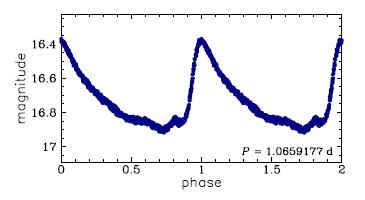
\includegraphics[width=\textwidth]{img/OGLE-LMC-CEP-2491.png}
		\small (a) Cefeida cl\'asica
	\end{minipage}
	\hfill
	\begin{minipage}{0.32\textwidth}
		\centering
		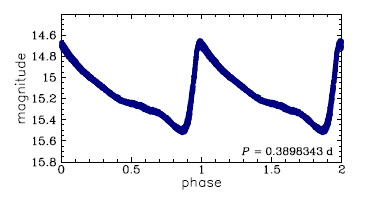
\includegraphics[width=\textwidth]{img/OGLE-BLG-RRLYR-09643.png}
		\small (b) RR Lyrae
	\end{minipage}
	\hfill
	\begin{minipage}{0.32\textwidth}
		\centering
		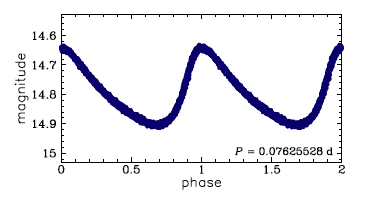
\includegraphics[width=\textwidth]{img/OGLE-BLG-DSCT-04672.png}
		\small (c) $\delta$~Scuti
	\end{minipage}
	\caption[Curvas de luz plegadas en fase de estrellas pulsantes]{Curvas de luz plegadas en fase de tres estrellas pulsantes del cat\'alogo de OGLE: (a) una Cefeida cl\'asica (OGLE-LMC-CEP-2491, $P=1.0659$~d), (b) una RR Lyrae (OGLE-BLG-RRLYR-09643, $P=0.3898$~d) y (c) una $\delta$~Scuti (OGLE-BLG-DSCT-04672, $P=0.0763$~d). En (a) y (b) se aprecia la rama ascendente, breve, en la que el brillo aumenta r\'apidamente hasta el m\'aximo, seguida de una rama descendente mucho m\'as prolongada en fase, en la que el brillo disminuye gradualmente hasta el m\'inimo; esta asimetr\'ia caracter\'istica es mucho menos marcada en la morfolog\'ia m\'as sim\'etrica y de menor amplitud de (c).}
	\label{fig:lc-pulsantes}
\end{figure}

\subsection{Binarias eclipsantes y variables elipsoidales}

A diferencia de las estrellas pulsantes, cuya variabilidad es intr\'inseca y est\'a determinada por su edad, masa y estado evolutivo, las binarias eclipsantes son sistemas de dos estrellas cuya variabilidad es puramente geom\'etrica: el brillo total del sistema cambia porque una componente oculta peri\'odicamente a la otra, vista desde la Tierra \citep{Karttunen2016}. La Figura~\ref{fig:lc-ecl-generica} muestra un ejemplo real de este comportamiento.

\begin{figure}[H]
	\centering
	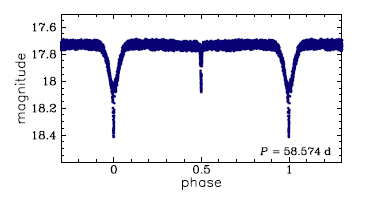
\includegraphics[width=0.5\textwidth]{img/OGLE-LMC-ECL-08181.png}
	\caption[Curva de luz de una binaria eclipsante]{Curva de luz plegada en fase de una binaria eclipsante del cat\'alogo de OGLE (OGLE-LMC-ECL-08181, $P=58.574$~d), tomada del \emph{OGLE Atlas of Variable Star Light Curves}. El brillo permanece esencialmente constante fuera de los eclipses, que son breves en relaci\'on con el periodo orbital.}
	\label{fig:lc-ecl-generica}
\end{figure}

Seg\'un la forma de su curva de luz, las binarias eclipsantes se agrupan tradicionalmente en tres tipos principales \citep{Karttunen2016}:

\begin{itemize}
	\item \textbf{Tipo Algol (EA)}, llamadas as\'i por $\beta$~Persei. Son sistemas separados (\emph{detached}), en los que ninguna componente llena su l\'obulo de Roche. La curva de luz es plana durante la mayor parte del periodo, con dos m\'inimos bien definidos, el primario notablemente m\'as profundo que el secundario.
	\item \textbf{Tipo $\beta$ Lyrae (EB)}. Son sistemas semiseparados, en los que una de las componentes ha llenado su l\'obulo de Roche y transfiere masa a la otra, adquiriendo una forma elipsoidal. El brillo total var\'ia de forma continua a lo largo de todo el periodo, no solo durante los eclipses.
	\item \textbf{Tipo W Ursae Majoris (EW)}. Son binarias de contacto, en las que ambas componentes llenan su l\'obulo de Roche y comparten una envoltura com\'un. Los dos m\'inimos de la curva de luz son casi id\'enticos en profundidad, anchos y redondeados, con periodos t\'ipicamente cortos, de menos de un d\'ia.
\end{itemize}

La Figura~\ref{fig:lc-ecl-subtipos} ilustra las diferencias morfol\'ogicas entre estos tres tipos con curvas de luz reales del cat\'alogo de OGLE.

\begin{figure}[H]
	\centering
	\begin{minipage}{0.32\textwidth}
		\centering
		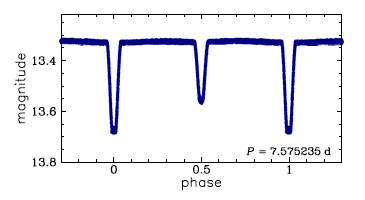
\includegraphics[width=\textwidth]{img/OGLE-BLG-ECL-126852-EA.png}
		\small (a) Algol (EA)
	\end{minipage}
	\hfill
	\begin{minipage}{0.32\textwidth}
		\centering
		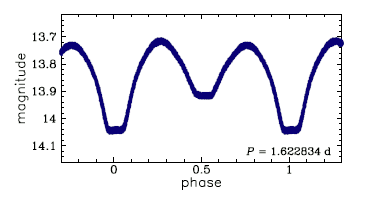
\includegraphics[width=\textwidth]{img/OGLE-BLG-ECL-217270-EB.png}
		\small (b) $\beta$ Lyrae (EB)
	\end{minipage}
	\hfill
	\begin{minipage}{0.32\textwidth}
		\centering
		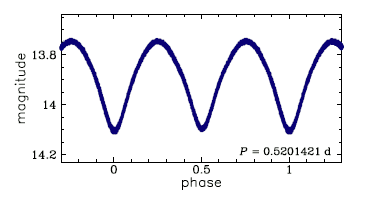
\includegraphics[width=\textwidth]{img/OGLE-BLG-ECL-163835-EW.png}
		\small (c) W Ursae Majoris (EW)
	\end{minipage}
	\caption[Curvas de luz de los tres tipos de binarias eclipsantes]{Curvas de luz plegadas en fase de los tres tipos morfol\'ogicos de binarias eclipsantes: (a) tipo Algol (OGLE-BLG-ECL-126852, $P=7.575$~d), con m\'inimos bien diferenciados y brillo constante fuera de ellos; (b) tipo $\beta$~Lyrae (OGLE-BLG-ECL-217270, $P=1.623$~d), con variaci\'on continua entre eclipses de profundidad desigual; y (c) tipo W~Ursae~Majoris (OGLE-BLG-ECL-163835, $P=0.520$~d), con m\'inimos casi id\'enticos y periodo corto.}
	\label{fig:lc-ecl-subtipos}
\end{figure}

Un tipo relacionado, que no presenta eclipses propiamente dichos, son las variables elipsoidales, en las que la deformaci\'on por marea de al menos una de las componentes hacia una forma elipsoidal produce una variaci\'on peri\'odica del \'area proyectada y, por tanto, del brillo, sin que exista un tr\'ansito real de una estrella frente a la otra \citep{Karttunen2016}. La Figura~\ref{fig:lc-ell} muestra un ejemplo real de este comportamiento.

\begin{figure}[H]
	\centering
	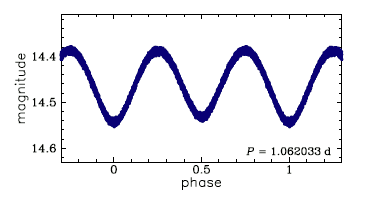
\includegraphics[width=0.5\textwidth]{img/OGLE-LMC-ECL-31518-ELL.png}
	\caption[Curva de luz de una variable elipsoidal]{Curva de luz plegada en fase de una variable elipsoidal del cat\'alogo de OGLE (OGLE-LMC-ECL-31518, $P=1.062$~d). A diferencia de las binarias eclipsantes de la Figura~\ref{fig:lc-ecl-subtipos}, la variaci\'on es suave y continua, sin m\'inimos abruptos.}
	\label{fig:lc-ell}
\end{figure}

A diferencia de las Cefeidas y las RR Lyrae, cuyo rango de periodos y ubicaci\'on en el diagrama HR est\'an determinados por un mecanismo pulsacional intr\'inseco ligado a su edad y masa, las binarias eclipsantes no pertenecen a una poblaci\'on estelar particular ni ocupan una regi\'on fija del diagrama HR: su periodo orbital, que puede ir desde unas pocas horas en sistemas de contacto hasta a\~nos en binarias separadas y anchas, depende principalmente de la separaci\'on entre las componentes y no de su edad evolutiva \citep{Karttunen2016}. Esto las convierte en un caso de prueba particularmente exigente para los m\'etodos de determinaci\'on de periodicidad, dado que combinan eclipses de corta duraci\'on relativa al periodo con formas de curva de luz muy alejadas de una sinusoide.

\subsection{Flujo general de b\'usqueda y caracterizaci\'on de estrellas variables}

M\'as all\'a del inter\'es en la f\'isica particular de cada tipo de variabilidad, la b\'usqueda sistem\'atica de estrellas variables en un cartografiado fotom\'etrico sigue, en t\'erminos generales, un flujo de trabajo com\'un. A partir de observaciones fotom\'etricas repetidas de un campo del cielo, se construye la serie temporal de cada objeto detectado como magnitud versus tiempo. Sobre esta serie de tiempo se calculan estad\'isticos que resumen su comportamiento, tales como el \'indice de variabilidad, la amplitud, o la asimetr\'ia de la distribuci\'on de magnitudes, con el fin de separar las estrellas genuinamente variables de aquellas que solo presentan ruido fotom\'etrico. Una vez identificado un objeto como variable, la determinaci\'on de su periodo resulta ser una de las variables m\'as decisivas para su clasificaci\'on posterior: el periodo, junto con la amplitud y la forma de la curva de luz plegada en fase, permite discriminar entre los distintos tipos de variabilidad descritos anteriormente, y constituye adem\'as, en el caso de Cefeidas y RR Lyrae, el insumo directo de las relaciones periodo--luminosidad utilizadas como indicadores de distancia. Por esta raz\'on, contar con determinaciones de periodo precisas y confiables no es solamente un fin en s\'i mismo, sino un paso habilitante para gran parte de la caracterizaci\'on posterior de una estrella variable.

\subsection{M\'etodos basados en el an\'alisis espectral}

El enfoque cl\'asico para la b\'usqueda de periodicidades en series de tiempo astron\'omicas es el an\'alisis de Fourier. Sin embargo, la mayor\'ia de las series de tiempo astron\'omicas est\'an muestreadas de forma irregular, debido a limitaciones observacionales como el ciclo d\'ia--noche, las fases lunares y las condiciones clim\'aticas. Esto impide la aplicaci\'on directa de la transformada discreta de Fourier cl\'asica. \citet{lomb_1976} y \citet{scargle_1982} resuelven este problema formulando la detecci\'on de periodicidad como un ajuste de m\'inimos cuadrados de una funci\'on sinusoidal para cada frecuencia de prueba. As\'i nace el periodograma de Lomb--Scargle: una generalizaci\'on del an\'alisis de Fourier, matem\'aticamente equivalente a este \'ultimo cuando el muestreo es uniforme. Esta t\'ecnica es, hasta la fecha, una de las m\'as utilizadas en la literatura. Su eficiencia computacional y su teor\'ia estad\'istica bien establecida, que permite evaluar la significancia de los picos del periodograma, explican su popularidad. Su principal limitaci\'on aparece cuando la variabilidad subyacente se aparta significativamente de una forma sinusoidal, como ocurre en eclipses pronunciados o en pulsaciones con arm\'onicos dominantes. En estos casos, la potencia espectral se fracciona entre la frecuencia fundamental y sus arm\'onicos, lo que dificulta identificar sin ambig\"uedad el periodo correcto. Su amplia adopci\'on se ve favorecida, adem\'as, por la disponibilidad de implementaciones computacionales maduras y de acceso libre: en este trabajo se emplear\'a la implementaci\'on del periodograma de Lomb--Scargle incluida en el paquete de Python \texttt{Astropy} \citep{astropy}.

\subsection{M\'etodos basados en el orden de fase}

Una familia alternativa de m\'etodos, menos sensible a la forma funcional de la se\~nal, se basa en evaluar el grado de orden que exhibe la curva de luz al ser plegada en fase para un periodo de prueba dado. Dentro de esta familia se encuentran t\'ecnicas como la minimizaci\'on de la dispersi\'on de fase (PDM) y el an\'alisis de varianza (AOV), popularizadas desde finales de la d\'ecada de 1970 \citep[v\'ease la revisi\'on de][]{Graham2013}. El m\'etodo de m\'inima entrop\'ia pertenece conceptualmente a esta familia. Fue propuesto por \citet{cincotta_1995} y formalizado anal\'iticamente por \citet{cincotta_1999}, y se distingue de los dem\'as m\'etodos de dispersi\'on de fase por sustentarse en un marco te\'orico riguroso proveniente de la teor\'ia de la informaci\'on: el periodo correcto es aquel que produce el diagrama de fase con menor entrop\'ia de Shannon, es decir, el de mayor orden estad\'istico. F\'isicamente, esto equivale a decir que el periodo correcto es aquel que ordena mejor los datos al plegarlos en fase, sin importar la forma que tenga esa curva ordenada. Esta formulaci\'on es intr\'insecamente sensible a cualquier morfolog\'ia de variabilidad, pues no exige asumir una forma funcional particular para la se\~nal. Por ello resulta especialmente adecuada para curvas de luz con eclipses, pulsaciones asim\'etricas o comportamientos multiperi\'odicos. A diferencia del periodograma de Lomb--Scargle, el m\'etodo de m\'inima entrop\'ia no cuenta con una implementaci\'on est\'andar de amplia difusi\'on; en este trabajo se emplear\'a \texttt{entropypf}, una implementaci\'on en Python de autor\'ia propia del autor de este trabajo.

\subsection{Comparaciones sistem\'aticas y limitaciones persistentes}

El trabajo de \citet{Graham2013} constituye la comparaci\'on sistem\'atica m\'as citada entre algoritmos de determinaci\'on de periodicidad, evaluando m\'etodos basados en Fourier, dispersi\'on de fase y entrop\'ia condicional sobre curvas de luz reales de los cartografiados Catalina Real-Time Transient Survey, MACHO y ASAS. Sus resultados muestran que los m\'etodos basados en dispersi\'on de fase y entrop\'ia condicional ofrecen consistentemente los mejores resultados en t\'erminos de completitud. Sin embargo, los autores se\~nalan expl\'icitamente que \emph{el aliasing de periodos y la identificaci\'on de arm\'onicos siguen siendo problemas significativos}, incluso para los m\'etodos m\'as precisos. Este hallazgo es central para la presente propuesta. Sugiere que la principal debilidad de los m\'etodos de orden de fase no es su precisi\'on una vez identificado el periodo correcto, sino la dificultad para descartar eficientemente picos esp\'ureos y arm\'onicos entre un gran n\'umero de periodos candidatos. Esta \'ultima es precisamente la tarea para la cual el periodograma de Lomb--Scargle, con su interpretaci\'on espectral directa, resulta m\'as id\'oneo.

M\'as recientemente, \citet{gurpide_2025} retomaron el problema de la detecci\'on de periodicidades en datos muestreados irregularmente. Se\~nalan que los periodogramas cl\'asicos carecen de propiedades estad\'isticas bien definidas bajo muestreo irregular, un problema que se agrava en presencia de variabilidad aperi\'odica o estoc\'astica (``ruido rojo''), f\'acilmente confundible con una se\~nal peri\'odica genuina. Su propuesta, basada en procesos gaussianos, confirma que el problema de la determinaci\'on robusta de periodicidad en datos irregulares dista de estar resuelto y que sigue siendo un \'area activa de investigaci\'on metodol\'ogica.

En el contexto local, \citet{Cubillos2021} realiz\'o, bajo la direcci\'on del mismo director de este trabajo, una comparaci\'on directa entre el m\'etodo de m\'inima entrop\'ia, un m\'etodo basado en Fourier (\texttt{fnpeaks}) y el periodograma de Lomb--Scargle, enfocada en determinar la cantidad m\'inima de puntos observacionales necesaria para reconstruir confiablemente el periodo de Cefeidas, RR Lyrae y binarias eclipsantes. Este antecedente directo confirma la viabilidad pr\'actica de trabajar con estos tres m\'etodos sobre curvas de luz de morfolog\'ias diversas, y aporta un precedente metodol\'ogico valioso para el dise\~no de las pruebas de validaci\'on de la presente propuesta.

\subsection{Aprendizaje autom\'atico como enfoque complementario}

En a\~nos recientes, la disponibilidad de cat\'alogos masivos de curvas de luz ha impulsado el uso de t\'ecnicas de aprendizaje autom\'atico para la clasificaci\'on de estrellas variables. \citet{PerezOrtiz2017}, en un trabajo desarrollado en la Universidad de los Andes, evaluaron clasificadores supervisados (bosques aleatorios, m\'aquinas de soporte vectorial, entre otros) para identificar candidatas a estrellas Be en el campo del polo ecl\'iptico sur de OGLE-IV. \citet{naydenkin_2020}, por su parte, aplicaron un enfoque similar para clasificar Cefeidas, RR Lyrae y estrellas $\delta$~Scuti en el cat\'alogo del Zwicky Transient Facility. En un trabajo m\'as reciente, tambi\'en desarrollado en la Universidad de los Andes, \citet{Elizabethson2023} entrenaron clasificadores supervisados sobre curvas de luz de TESS para distinguir morfolog\'ias asociadas a distintos mecanismos f\'isicos en estrellas T~Tauri j\'ovenes, ilustrando la extensi\'on de este tipo de enfoques a otros cartografiados y tipos de variabilidad. Es importante notar que estos m\'etodos abordan un problema distinto al de esta propuesta: la \emph{clasificaci\'on} de tipos de variabilidad a partir de caracter\'isticas extra\'idas de la curva de luz, en muchos casos incluyendo el periodo ya determinado por otros m\'etodos como una de dichas caracter\'isticas. En contraste, este trabajo se concentra en la \emph{determinaci\'on} misma del periodo, un paso previo y frecuentemente indispensable para dicha clasificaci\'on. La naturaleza de caja negra de los clasificadores de aprendizaje autom\'atico contrasta, adem\'as, con la interpretabilidad anal\'itica que ofrecen tanto el periodograma de Lomb--Scargle como el m\'etodo de m\'inima entrop\'ia. Esta es una caracter\'istica deseable cuando se busca comprender f\'isicamente el origen de la variabilidad detectada.

\subsection{Cartografiados observacionales contempor\'aneos}

La motivaci\'on observacional de este trabajo est\'a directamente ligada al estado actual de los grandes cartografiados fotom\'etricos. El proyecto OGLE, actualmente en su cuarta fase, mantiene el \emph{OGLE Collection of Variable Stars} \citep{iwanek_2025,soszynski_2024}. Se trata de un cat\'alogo p\'ublico y sistem\'aticamente ampliado de curvas de luz en las bandas $V$ e $I$, que cubre el bulbo de la V\'ia L\'actea y el disco de la V\'ia L\'actea, as\'i como el sistema de las Nubes de Magallanes, e incluye subcat\'alogos espec\'ificos para Cefeidas, RR Lyrae y binarias eclipsantes, entre otros tipos de variabilidad \citep{Soszynski2008,Soszynski2009,Soszynski2010,Soszynski2010b,Soszynski2011,Soszynski2011b,Soszynski2014,Soszynski2016,pawlak2016,pietrukowicz2013b}. El cartografiado VVV y su extensi\'on VVVX complementan esta cobertura en el infrarrojo cercano, proporcionando fotometr\'ia $JHK_s$ para regiones de alta extinci\'on interestelar inaccesibles en el \'optico \citep{vvv_survey,saito_2024}. La misi\'on espacial TESS, dise\~nada originalmente para la detecci\'on de exoplanetas en tr\'ansito, aporta finalmente fotometr\'ia de cadencia de pocos minutos y l\'ineas base continuas de semanas a meses \citep{ricker_2015}. Estas cualidades la han convertido en una fuente cada vez m\'as explotada para la determinaci\'on de periodos de estrellas variables en general, no solo de sistemas con planetas en tr\'ansito, como lo demuestra el trabajo reciente de \citet{kepler_2026} sobre periodos fotom\'etricos de variables catacl\'ismicas.

\section{Motivaci\'on y justificaci\'on}
\label{sec:motivacion}

De la revisi\'on anterior se desprende un panorama consistente. El periodograma de Lomb--Scargle es computacionalmente eficiente y concentra su poder estad\'istico en identificar frecuencias dominantes, pero fracciona su sensibilidad ante se\~nales con arm\'onicos importantes. El m\'etodo de m\'inima entrop\'ia, en cambio, es sensible a cualquier morfolog\'ia de variabilidad; sin embargo, como lo evidenci\'o \citet{Graham2013}, el aliasing y la identificaci\'on del arm\'onico correcto siguen siendo problemas persistentes incluso para los m\'etodos de orden de fase m\'as precisos. Estas debilidades no son independientes entre s\'i. La principal fortaleza de Lomb--Scargle, su capacidad de identificar eficientemente las frecuencias f\'isicamente relevantes dentro de un espacio de b\'usqueda amplio mediante una sola pasada vectorizada, es precisamente la herramienta que se necesita para mitigar la principal debilidad del m\'etodo de entrop\'ia m\'inima.

Con base en esto, se propone construir un m\'etodo combinado en el que el periodograma de Lomb--Scargle y el criterio de m\'inima entrop\'ia se apliquen en paralelo, de forma simult\'anea, sobre la misma grilla de periodos de prueba, y no uno como filtro previo del otro. El periodo final candidato se obtiene combinando ambos criterios, favoreciendo los periodos que exhiban simult\'aneamente alta potencia espectral y baja entrop\'ia. La hip\'otesis central de este trabajo es que esta integraci\'on paralela permite superar las limitaciones de cada t\'ecnica por separado. La capacidad de discriminaci\'on de frecuencias del periodograma, combinada con la robustez morfol\'ogica del criterio de entrop\'ia, deber\'ia producir determinaciones de periodo m\'as precisas y m\'as robustas que cualquiera de los dos m\'etodos aplicados de forma individual.

\section{Objetivo general}
\label{sec:objetivo-general}

Desarrollar y validar un m\'etodo para la determinaci\'on robusta de periodos en estrellas variables mediante la integraci\'on del periodograma de Lomb--Scargle y el criterio de m\'inima entrop\'ia, aplicado a curvas de luz con distintas morfolog\'ias de variabilidad.

\section{Objetivos espec\'ificos}
\label{sec:objetivos-especificos}

\begin{itemize}
	\item Implementar de manera independiente el periodograma de Lomb--Scargle y el m\'etodo de m\'inima entrop\'ia, caracterizando sus fortalezas y limitaciones frente a diferentes tipos de variabilidad estelar.
	\item Dise\~nar un esquema de integraci\'on entre ambas t\'ecnicas que permita identificar de forma consistente el periodo y la fase m\'as probables en curvas de luz.
	\item Evaluar el desempe\~no del m\'etodo propuesto utilizando curvas de luz sint\'eticas con distintas morfolog\'ias f\'isicas, niveles de ruido y cadencias de muestreo.
	\item Comparar la precisi\'on y robustez del m\'etodo desarrollado frente a la aplicaci\'on individual de Lomb--Scargle y m\'inima entrop\'ia en datos reales de los proyectos OGLE, VVV y TESS.
\end{itemize}


\chapter{Descripci\'on de los datos}
\label{ch:datos}

Para dise\~nar, entrenar el criterio de decisi\'on y validar el m\'etodo combinado propuesto en este trabajo se emplear\'an dos categor\'ias de datos. La primera son curvas de luz sint\'eticas, generadas con control total sobre la morfolog\'ia de la se\~nal, el nivel de ruido y la cadencia de muestreo. La segunda son curvas de luz reales, provenientes de los cartografiados OGLE, VVV/VVVX y TESS, cuyos periodos catalogados sirven como referencia (\emph{ground truth}) independiente. Este cap\'itulo describe ambas fuentes de datos.

\section{Curvas de luz sint\'eticas}
\label{sec:datos-sinteticas}

El uso de curvas de luz sint\'eticas permite evaluar el desempe\~no de un algoritmo de determinaci\'on de periodicidad bajo condiciones completamente controladas, en las que el periodo verdadero es conocido de antemano. Esta estrategia fue empleada originalmente por \citet{cincotta_1995} para validar el m\'etodo de m\'inima entrop\'ia, y ser\'a adoptada aqu\'i con tres grados de libertad principales: la morfolog\'ia f\'isica de la variabilidad, el modelo de ruido, y la cadencia de muestreo temporal.

Esta estrategia complementa, en lugar de reemplazar, el uso de datos reales, y resulta indispensable por al menos tres razones. En primer lugar, en los datos reales el periodo verdadero de una estrella no se conoce con certeza absoluta, sino que proviene, a su vez, de la aplicaci\'on de alg\'un otro m\'etodo de determinaci\'on de periodicidad reportado en la literatura; esto introduce una circularidad que las curvas sint\'eticas, con periodo impuesto por construcci\'on, evitan por completo. En segundo lugar, las curvas de luz reales combinan de forma simult\'anea e inseparable la morfolog\'ia de la variabilidad, el nivel de ruido y el patr\'on de muestreo, lo que dificulta atribuir un cambio en el desempe\~no de un m\'etodo a una causa espec\'ifica; las curvas sint\'eticas permiten, en cambio, variar cada uno de estos factores de forma independiente y sistem\'atica. En tercer lugar, las curvas sint\'eticas permiten explorar regiones del espacio de par\'ametros, como niveles de ruido extremos o cadencias de muestreo particularmente escasas, que pueden estar subrepresentadas o ausentes en los cat\'alogos reales disponibles, pero que son relevantes para caracterizar los l\'imites de aplicabilidad del m\'etodo combinado.

\subsection{Morfolog\'ias de variabilidad}

Se generar\'an tres familias de curvas de luz sint\'eticas, representativas de los principales mecanismos f\'isicos de variabilidad estelar discutidos en la Secci\'on~\ref{sec:estado-del-arte}:

\begin{itemize}
	\item \textbf{Oscilaciones sinusoidales}, como aproximaci\'on de primer orden a pulsadores radiales de baja amplitud, representadas por una \'unica componente arm\'onica.
	\item \textbf{Pulsaciones asim\'etricas}, representativas de Cefeidas y RR Lyrae cl\'asicas, cuyas curvas de luz reales exhiben una rama ascendente breve hacia el m\'aximo de brillo, seguida de una rama descendente m\'as prolongada hacia el m\'inimo, y que se modelar\'an mediante una serie de Fourier truncada con m\'ultiples arm\'onicos y fases relativas no triviales entre ellos \citep{Karttunen2016,Carroll2017}.
	\item \textbf{Eclipses}, representativos de sistemas binarios eclipsantes, caracterizados por m\'inimos de brillo abruptos y de corta duraci\'on relativa al periodo orbital, que fraccionan fuertemente la potencia espectral entre la frecuencia fundamental y sus arm\'onicos al ser analizados mediante t\'ecnicas puramente espectrales.
\end{itemize}

Esta selecci\'on de morfolog\'ias permite explorar de manera controlada el espacio en el que se espera que las fortalezas y debilidades de Lomb--Scargle y de la entrop\'ia m\'inima sean m\'as distinguibles. Se anticipa que ambos m\'etodos se desempe\~nen de forma similar sobre la morfolog\'ia sinusoidal, mientras que las morfolog\'ias asim\'etrica y de eclipses deber\'ian favorecer progresivamente al m\'etodo de entrop\'ia.

\subsection{Modelo de ruido}

Adem\'as del ruido blanco gaussiano, que aproxima el ruido fotom\'etrico y de conteo de fotones, se incorporar\'a ruido correlacionado (``ruido rojo'', o ruido con espectro de potencias tipo ley de potencia). Para esto se usar\'a el algoritmo de \citet{timmer_1995}, que genera series de tiempo estoc\'asticas con un espectro de potencias prescrito, aleatorizando tanto la fase como la amplitud de la transformada de Fourier de la se\~nal. \citet{gurpide_2025} se\~nalan que la variabilidad aperi\'odica de tipo ruido rojo es f\'acilmente confundible con una se\~nal peri\'odica genuina cuando se emplean periodogramas cl\'asicos. Por esta raz\'on, su inclusi\'on constituye una prueba de robustez exigente para cualquier m\'etodo de determinaci\'on de periodicidad.

\subsection{Cadencia y muestreo temporal}

Finalmente, cada combinaci\'on de morfolog\'ia y nivel de ruido se muestrear\'a bajo distintos esquemas temporales: muestreo regular denso, como referencia; y muestreo irregular con brechas, dise\~nado para emular las ventanas de visibilidad estacional y las interrupciones diarias t\'ipicas de los cartografiados terrestres descritos en la Secci\'on~\ref{sec:datos-reales}. Este \'ultimo esquema es central para poner a prueba el comportamiento de ambos m\'etodos frente al aliasing, cuya relaci\'on con la frecuencia de Nyquist bajo muestreo irregular se discute con mayor detalle en la Secci\'on~\ref{sec:nyquist} del Cap\'itulo~\ref{ch:metodologia}.

\section{Curvas de luz reales}
\label{sec:datos-reales}

\subsection{OGLE}

El \emph{Optical Gravitational Lensing Experiment} (OGLE)\footnote{P\'agina web del proyecto: \url{https://ogle.astrouw.edu.pl/}} es uno de los cartografiados fotom\'etricos m\'as extensos y longevos en operaci\'on \citep{soszynski_2024}. Naci\'o en 1992 y se ha desarrollado desde entonces en cuatro fases sucesivas, cada una con instrumentaci\'on progresivamente m\'as capaz, como se resume en la Tabla~\ref{tab:ogle-fases}.

\begin{table}[H]
	\centering
	\begin{tabular}{p{2.8cm}p{1.6cm}p{1.6cm}p{2.0cm}p{3.9cm}}
		\hline
		\textbf{Fase} & \textbf{C\'amara} & \textbf{\'Area (deg\textsuperscript{2})} & \textbf{Estrellas (millones)} & \textbf{Campo principal} \\
		\hline
		OGLE-I \newline (1992--1995) & 4~Mpx & 1.5 & 6 & Bulbo gal\'actico \\
		OGLE-II \newline (1997--2000) & 4~Mpx & 27 & 44 & Bulbo, Nubes de Magallanes \\
		OGLE-III \newline (2001--2009) & 64~Mpx & 170 & 389 & Bulbo, Nubes de Magallanes \\
		OGLE-IV \newline (2010--presente) & 256~Mpx & 3600 & 2000 & Bulbo, disco, Nubes de Magallanes \\
		\hline
	\end{tabular}
	\caption[Fases del proyecto OGLE]{Fases sucesivas del proyecto OGLE, con el tama\~no de la c\'amara utilizada, el \'area de cielo cubierta, el n\'umero aproximado de estrellas monitoreadas y el campo principal observado en cada una \citep{soszynski_2024}.}
	\label{tab:ogle-fases}
\end{table}

Las observaciones de OGLE-I se realizaron con el telescopio Swope de 1~m del Observatorio de Las Campanas, Chile. Desde OGLE-II, el proyecto ha empleado en cambio un telescopio dedicado de 1.3~m, tambi\'en ubicado en Las Campanas \citep{soszynski_2024}. A lo largo de sus cuatro fases, el proyecto ha acumulado m\'as de un bill\'on de observaciones fotom\'etricas individuales para aproximadamente dos mil millones de estrellas \citep{soszynski_2024,iwanek_2025}, principalmente en las bandas $V$ e $I$ del sistema Johnson--Cousins \citep{Bessell2005}. De particular inter\'es para este trabajo es el \emph{OGLE Collection of Variable Stars} (OCVS): un cat\'alogo p\'ublico que incluye fotometr\'ia en dichas bandas junto con los periodos catalogados de cientos de miles de estrellas variables, organizados en subcat\'alogos por tipo de variabilidad, incluyendo Cefeidas cl\'asicas, RR Lyrae y binarias eclipsantes \citep{Soszynski2008,Soszynski2009,Soszynski2010,Soszynski2010b,Soszynski2011,Soszynski2011b,Soszynski2014,Soszynski2016,pawlak2016,pietrukowicz2013b}. Estos periodos fueron obtenidos por el equipo de OGLE mediante procedimientos independientes de los que se emplear\'an en este trabajo. Por ello, constituyen una referencia externa contra la cual contrastar los resultados del m\'etodo combinado.

Con el fin de caracterizar mejor la composici\'on del subconjunto de OCVS relevante para este trabajo, se realiz\'o un sondeo descriptivo de los cat\'alogos de Cefeidas cl\'asicas, RR Lyrae y binarias del OCVS. La Figura~\ref{fig:ogle-totales} muestra el n\'umero total de estrellas catalogadas de cada tipo, junto con la fracci\'on de ellas para la cual existe fotometr\'ia individual disponible.

\begin{figure}[H]
	\centering
	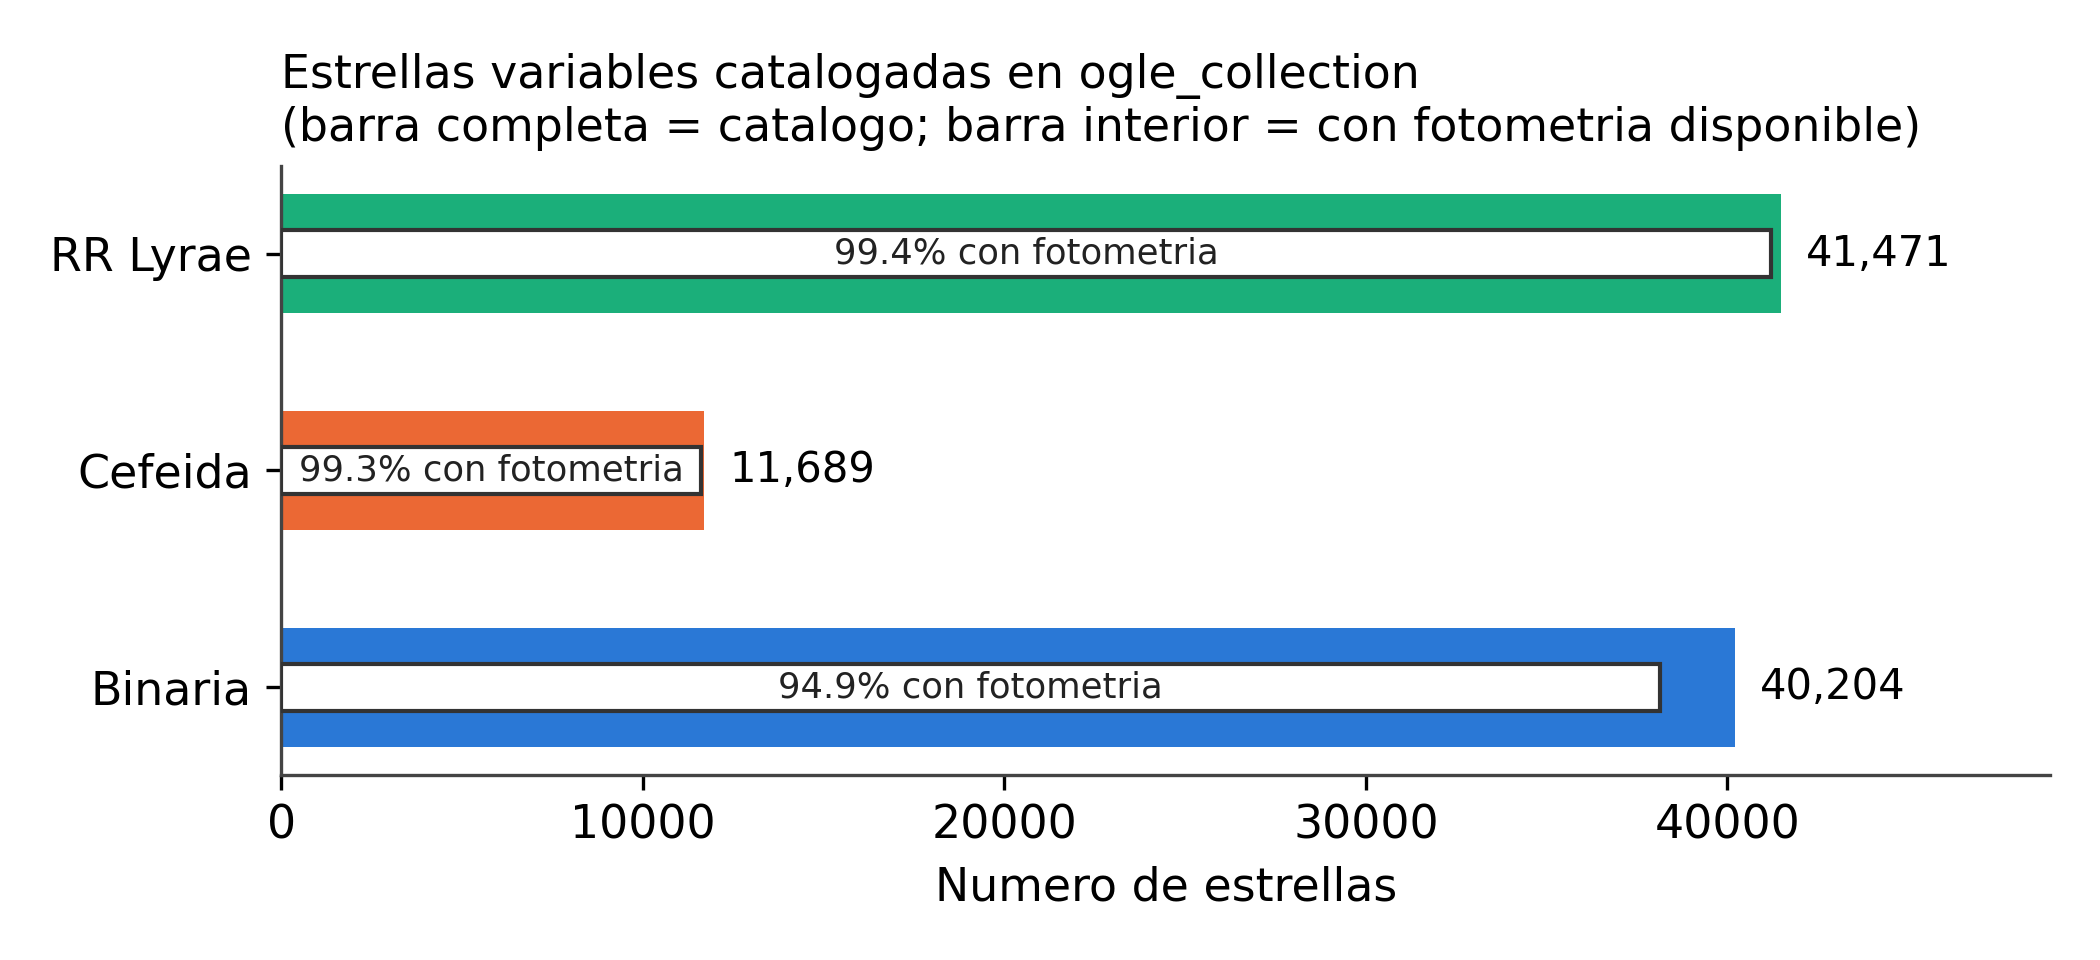
\includegraphics[width=0.85\textwidth]{img/ogle_totales_por_tipo.png}
	\caption[Estrellas del subconjunto de OCVS utilizado en este trabajo, por tipo]{N\'umero de estrellas, para cada uno de los tres tipos de variabilidad de inter\'es, dentro de los subcat\'alogos del OCVS descargados para el desarrollo de este trabajo, junto con la fracci\'on de ellas con fotometr\'ia individual disponible. Elaboraci\'on propia a partir de los cat\'alogos de \citet{Soszynski2008,Soszynski2009,Soszynski2010,Soszynski2010b,Soszynski2011,Soszynski2011b,Soszynski2014,Soszynski2016,pawlak2016,pietrukowicz2013b}.}
	\label{fig:ogle-totales}
\end{figure}

Las RR Lyrae y las binarias eclipsantes son, con much\'isima diferencia, los tipos de variabilidad m\'as numerosos en el subconjunto de OCVS considerado, mientras que las Cefeidas cl\'asicas son casi cuatro veces menos numerosas que cualquiera de los otros dos tipos. En los tres casos, la fracci\'on de estrellas con fotometr\'ia individual disponible supera el 94\%, lo cual garantiza una muestra amplia de curvas de luz reales sobre la cual aplicar el m\'etodo combinado.

La distribuci\'on espacial de estas estrellas tambi\'en es marcadamente distinta entre tipos, como se aprecia en la Figura~\ref{fig:ogle-campo}.

\begin{figure}[H]
	\centering
	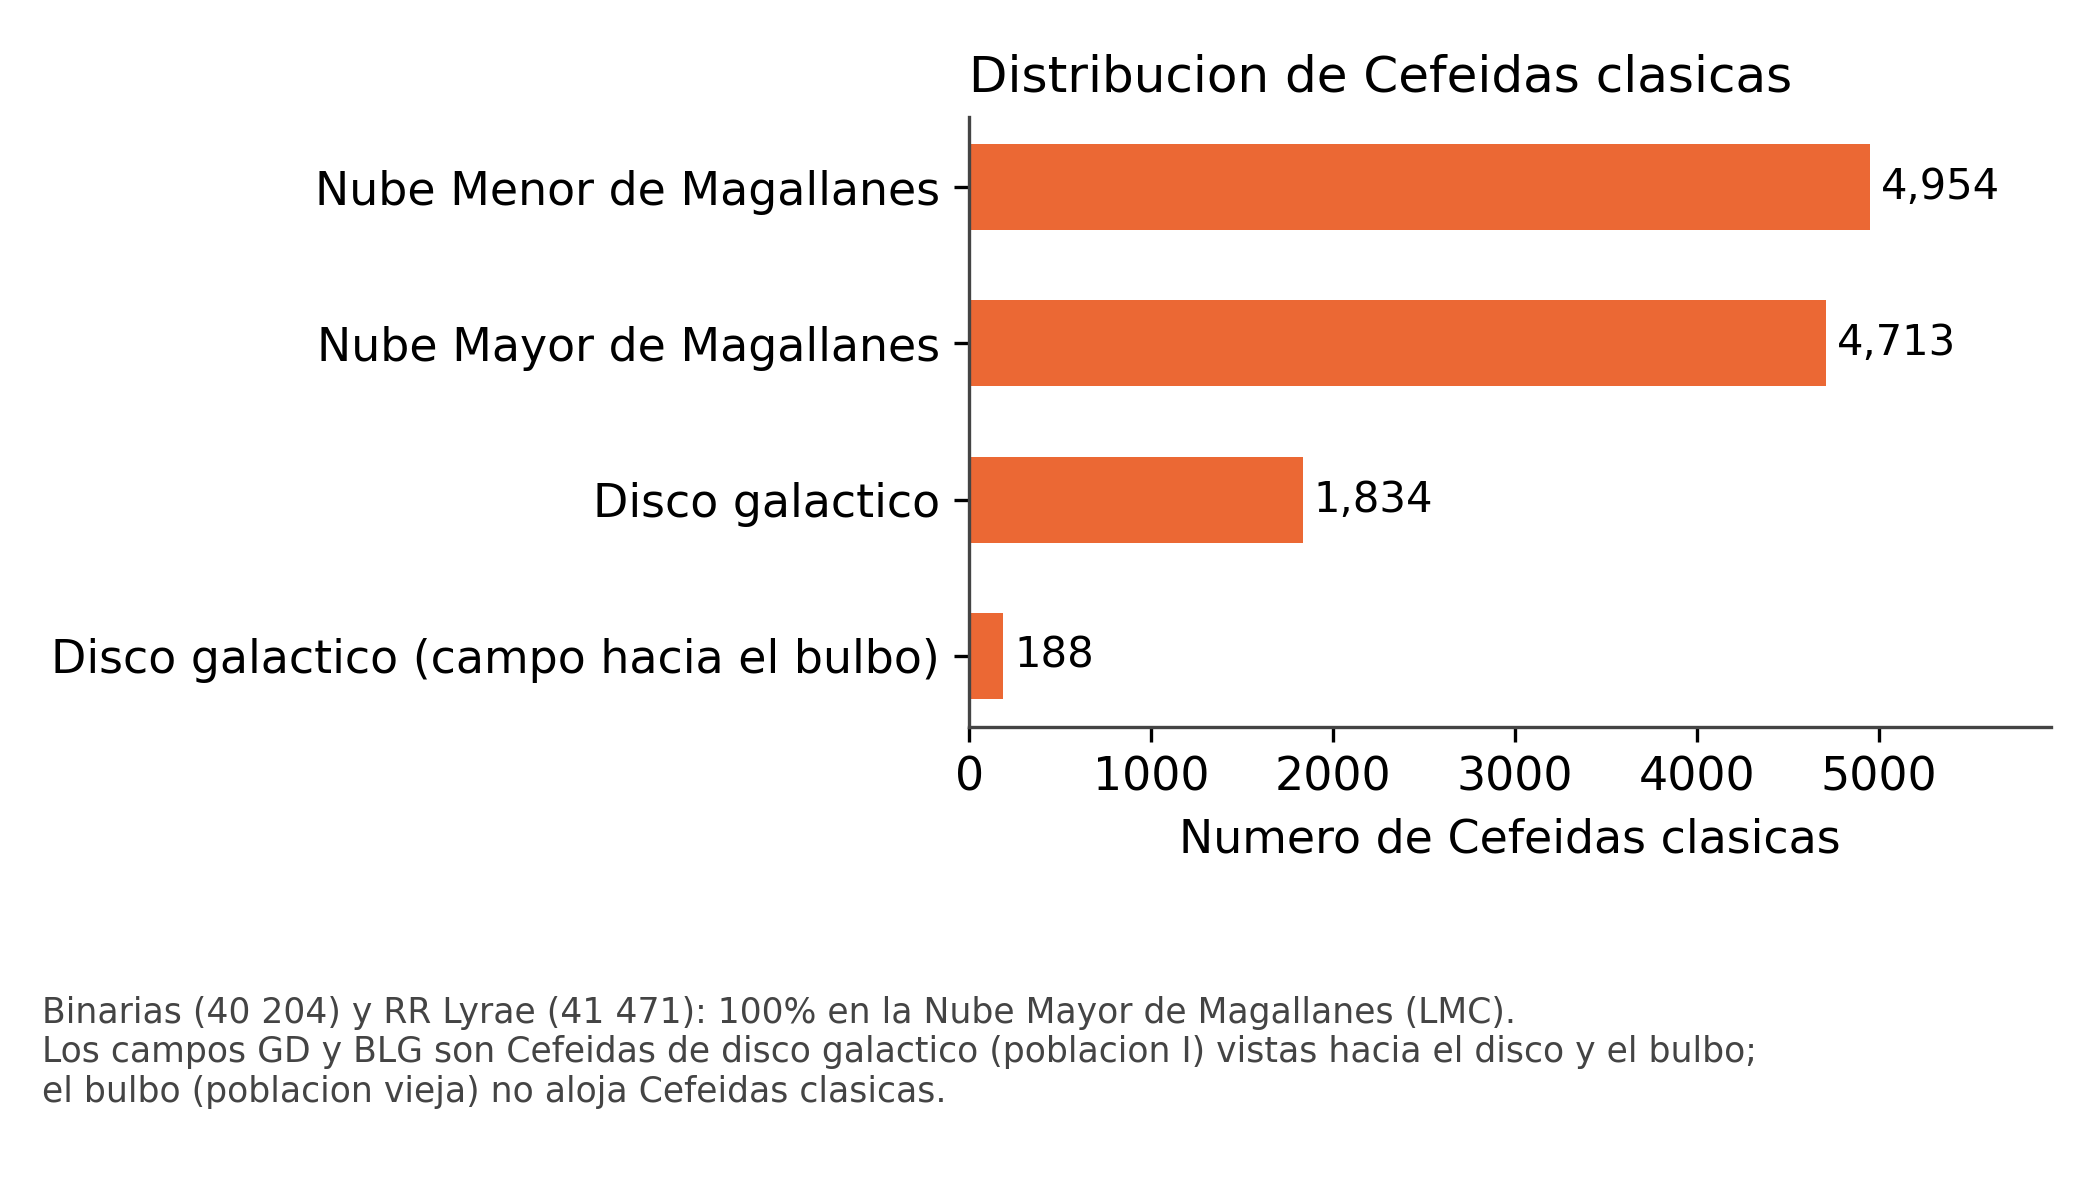
\includegraphics[width=0.85\textwidth]{img/ogle_distribucion_por_campo.png}
	\caption[Distribuci\'on de las Cefeidas cl\'asicas del subconjunto de OCVS utilizado]{Distribuci\'on, seg\'un la regi\'on observada, de las Cefeidas cl\'asicas incluidas en los subcat\'alogos del OCVS descargados para este trabajo. Todas las RR Lyrae y binarias eclipsantes de dichos subcat\'alogos se ubican en la Nube Mayor de Magallanes. Elaboraci\'on propia a partir de los cat\'alogos citados en la Figura~\ref{fig:ogle-totales}.}
	\label{fig:ogle-campo}
\end{figure}

Tanto las RR Lyrae como las binarias eclipsantes de este subconjunto se ubican en su totalidad en la Nube Mayor de Magallanes, mientras que las Cefeidas cl\'asicas se distribuyen entre ambas Nubes de Magallanes y el disco de la V\'ia L\'actea, incluyendo un peque\~no n\'umero de campos observados hacia el bulbo de la V\'ia L\'actea. Esto es consistente con lo discutido en la Secci\'on~\ref{sec:estado-del-arte}: al ser j\'ovenes trazadoras de poblaci\'on~I, las Cefeidas cl\'asicas se encuentran preferentemente en regiones de formaci\'on estelar reciente como el disco de la V\'ia L\'actea y las Nubes de Magallanes, y no en el bulbo de la V\'ia L\'actea, dominado por poblaci\'on vieja.

Dentro de las Cefeidas cl\'asicas, el cat\'alogo de OGLE reporta adem\'as el modo de pulsaci\'on identificado para cada estrella, lo cual permite contrastar directamente la discusi\'on te\'orica de la Secci\'on~\ref{sec:estado-del-arte} con datos observacionales, como se muestra en la Figura~\ref{fig:ogle-modos}.

\begin{figure}[H]
	\centering
	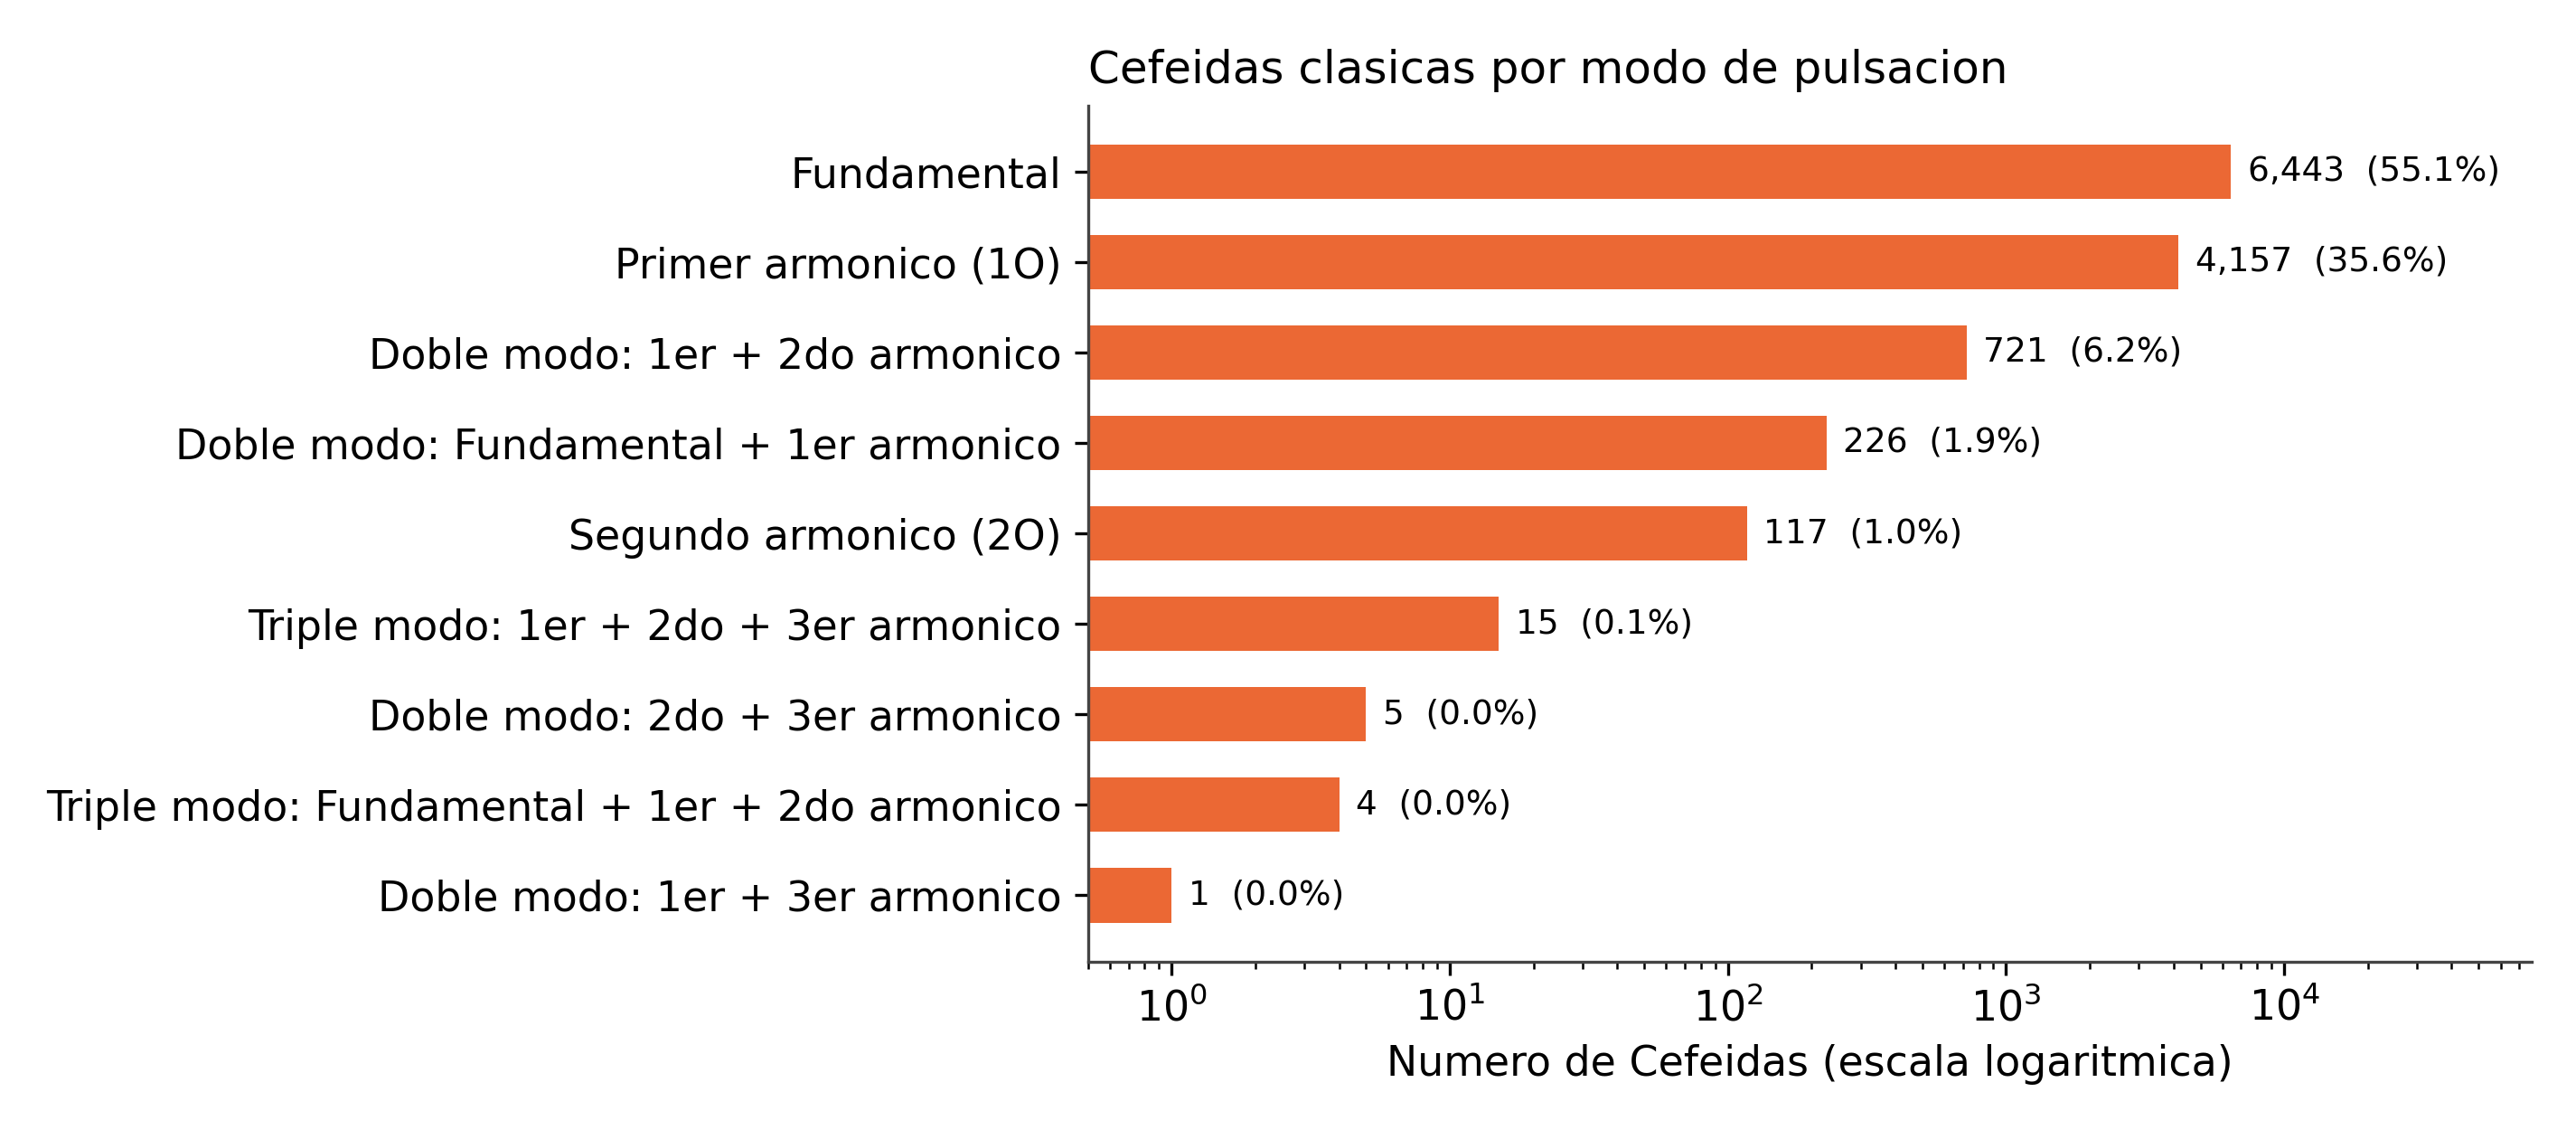
\includegraphics[width=0.85\textwidth]{img/ogle_cefeidas_por_modo.png}
	\caption[Cefeidas cl\'asicas del subconjunto de OCVS utilizado, por modo de pulsaci\'on]{Cefeidas cl\'asicas de los subcat\'alogos del OCVS descargados para este trabajo, seg\'un su modo de pulsaci\'on identificado. Elaboraci\'on propia a partir de los cat\'alogos citados en la Figura~\ref{fig:ogle-totales}.}
	\label{fig:ogle-modos}
\end{figure}

Consistentemente con lo se\~nalado por \citet{Carroll2017}, la gran mayor\'ia de las Cefeidas cl\'asicas del cat\'alogo pulsan en el modo fundamental (55.1\%) o en el primer sobretono (35.6\%), mientras que los modos m\'ultiples (doble o triple modo, que involucran combinaciones del modo fundamental con el primer, segundo o tercer arm\'onico) son considerablemente m\'as raros, y suman en conjunto menos del 10\% del cat\'alogo. Esta distribuci\'on tiene una implicaci\'on directa sobre la metodolog\'ia: las curvas de luz de Cefeidas de modo m\'ultiple contienen, por construcci\'on, m\'as de una periodicidad simult\'anea, lo cual constituye un caso de prueba adicionalmente exigente para los m\'etodos de determinaci\'on de periodicidad descritos en el Cap\'itulo~\ref{ch:metodologia}.

Finalmente, la Figura~\ref{fig:ogle-binarias} muestra la composici\'on del subcat\'alogo de binarias eclipsantes disponible para este trabajo, seg\'un su tipo morfol\'ogico, tal como lo reporta OGLE.

\begin{figure}[H]
	\centering
	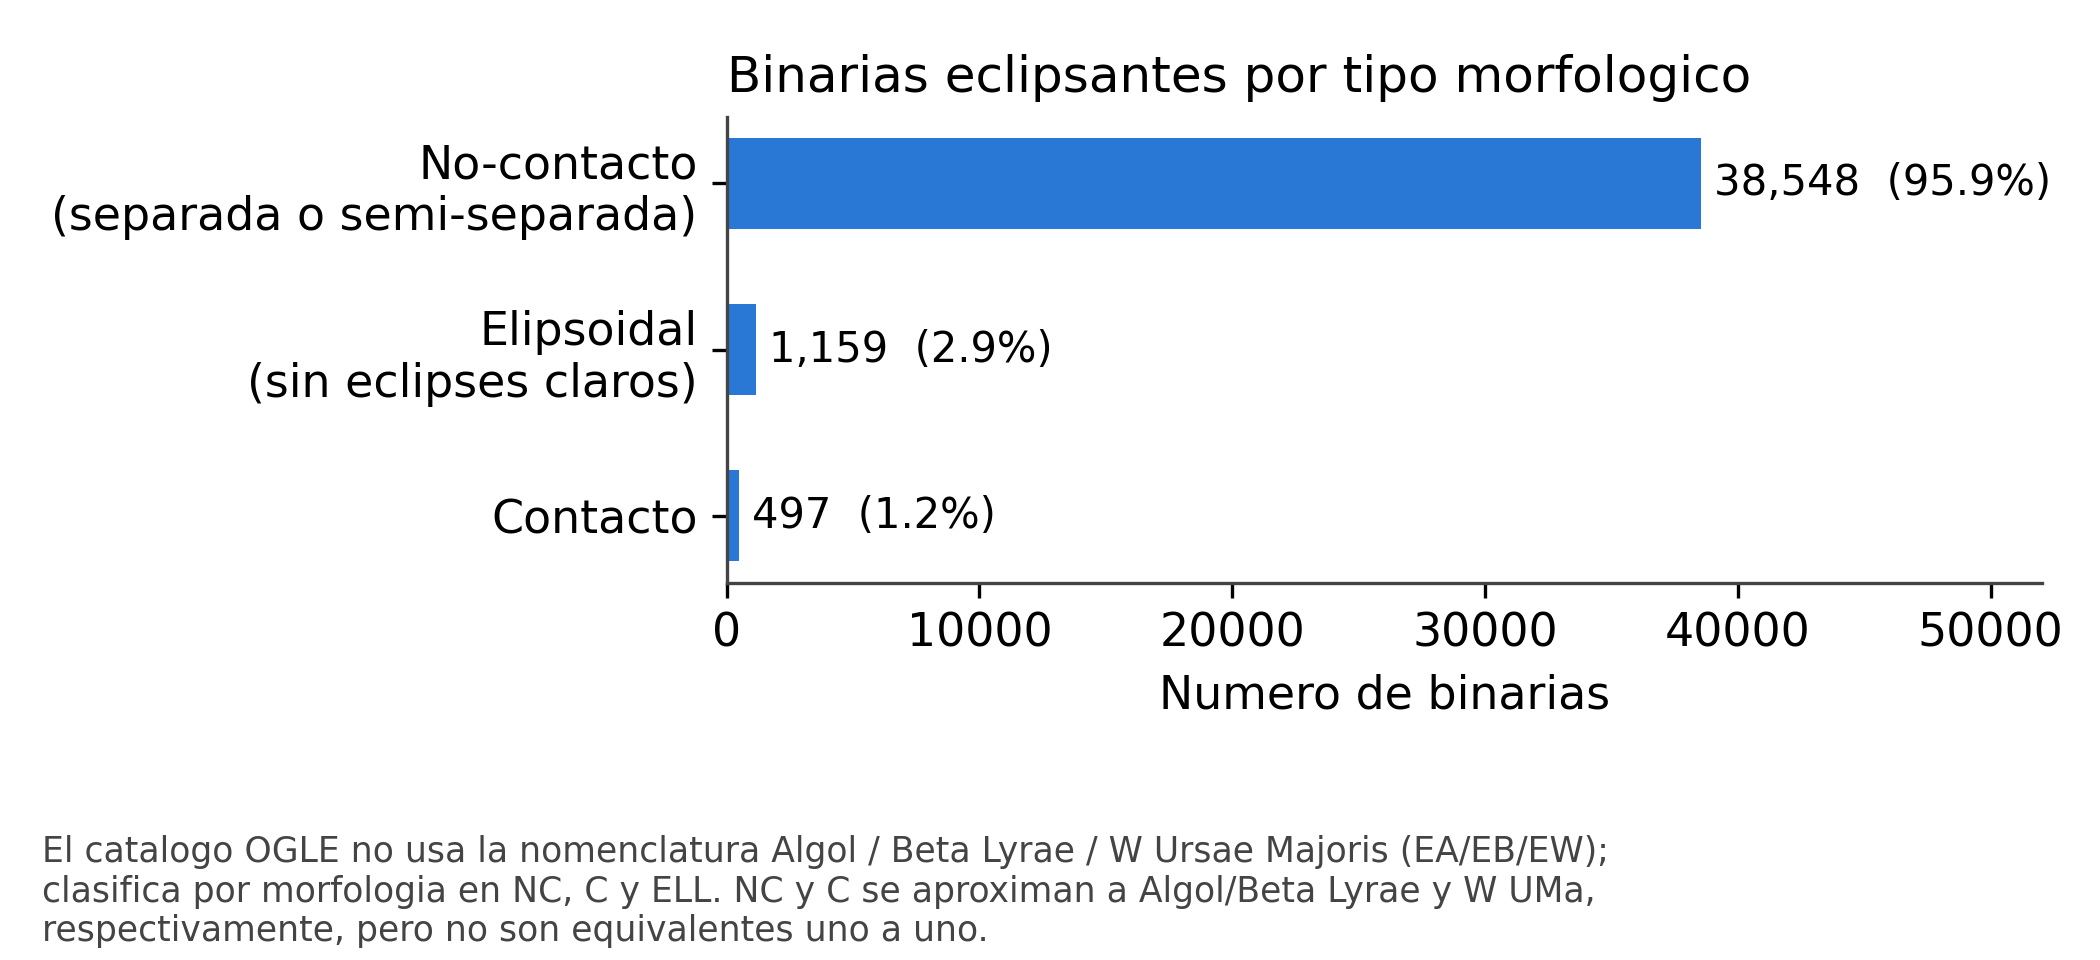
\includegraphics[width=0.85\textwidth]{img/ogle_binarias_por_tipo.png}
	\caption[Binarias eclipsantes del subconjunto de OCVS utilizado, por tipo morfol\'ogico]{Binarias eclipsantes de los subcat\'alogos del OCVS descargados para este trabajo, seg\'un su tipo morfol\'ogico. El cat\'alogo de OGLE clasifica las binarias como no-contacto (NC), contacto (C) o elipsoidal (ELL), en lugar de la nomenclatura Algol/$\beta$~Lyrae/W~Ursae~Majoris utilizada en la Secci\'on~\ref{sec:estado-del-arte}. Elaboraci\'on propia a partir de los cat\'alogos citados en la Figura~\ref{fig:ogle-totales}.}
	\label{fig:ogle-binarias}
\end{figure}

Es importante notar que la nomenclatura morfol\'ogica del cat\'alogo de OGLE no coincide exactamente con la clasificaci\'on cl\'asica de Algol, $\beta$~Lyrae y W~Ursae~Majoris introducida en la Secci\'on~\ref{sec:estado-del-arte}, sino que distingue entre sistemas de no-contacto (NC, que incluyen tanto binarias separadas como semiseparadas), de contacto (C) y elipsoidales (ELL, sin eclipses claros). Los sistemas de no-contacto, aproximadamente equivalentes a los tipos Algol y $\beta$~Lyrae, dominan ampliamente el cat\'alogo con un 95.9\% de las binarias, mientras que los sistemas de contacto, aproximadamente equivalentes al tipo W~Ursae~Majoris, representan apenas un 1.2\%; la correspondencia entre ambas clasificaciones, sin embargo, no es exactamente uno a uno. Dado que los sistemas de contacto son precisamente los que presentan las curvas de luz m\'as suaves y de periodo m\'as corto, su baja representaci\'on relativa en el cat\'alogo deber\'a tenerse en cuenta al seleccionar la muestra de binarias eclipsantes con la que se validar\'a el m\'etodo combinado sobre datos reales.

\subsection{VVV y VVVX}

El cartografiado \emph{VISTA Variables in the V\'ia L\'actea} (VVV)\footnote{P\'agina web del proyecto: \url{https://vvvsurvey.org/}} es un relevamiento p\'ublico del Observatorio Europeo Austral. Observa el bulbo de la V\'ia L\'actea y una secci\'on adyacente de su disco con el instrumento VIRCAM del telescopio VISTA de 4~m, en cinco bandas del infrarrojo cercano ($Z=0.87$, $Y=1.02$, $J=1.25$, $H=1.65$ y $K_s=2.14\ \mu$m) \citep{vvv_survey,Fajardo2026}. La regi\'on original de $562$ grados cuadrados se cubri\'o con una cadencia de aproximadamente 70 \'epocas por campo a lo largo de una l\'inea base de seis a\~nos (2010--2016), acumulando fotometr\'ia para m\'as de 288 millones de fuentes con una precisi\'on mejor a 0.05 magnitudes para estrellas con $K_s\lesssim16$ \citep{Fajardo2026}. Su extensi\'on, VVVX, ampli\'o la cobertura espacial original de $562$ a $1700$ grados cuadrados y a\~nadi\'o \'epocas adicionales de observaci\'on entre 2016 y 2023. Entre ambos cartografiados se acumularon aproximadamente $4200$ horas de observaci\'on, con las que se produjo un cat\'alogo de fuentes variables en banda $K_s$ del orden de $10^7$ objetos \citep{saito_2024}. La cobertura en el infrarrojo cercano hace de VVV/VVVX una fuente de datos complementaria a OGLE: la extinci\'on interestelar en banda $K_s$ es aproximadamente una d\'ecima parte de la extinci\'on en banda $V$ ($A_{K_s}/A_V\sim0.1$), lo cual permite penetrar regiones de alta extinci\'on interestelar donde la fotometr\'ia \'optica se ve fuertemente afectada \citep{Fajardo2026}. En contraste con OGLE, la cadencia de observaci\'on de VVV/VVVX es t\'ipicamente m\'as dispersa e irregular, con decenas de \'epocas repartidas a lo largo de varios a\~nos en lugar de observaciones casi diarias. Esto la convierte en un caso de prueba exigente para la determinaci\'on de periodicidad bajo muestreo irregular.

\subsection{TESS}

El \emph{Transiting Exoplanet Survey Satellite} (TESS)\footnote{P\'agina web del proyecto: \url{https://tess.mit.edu/}} es una misi\'on espacial de la NASA de la clase Explorer, dise\~nada originalmente para la detecci\'on de exoplanetas en tr\'ansito alrededor de estrellas brillantes y cercanas \citep{ricker_2015}. Emplea cuatro c\'amaras CCD de campo amplio en una \'orbita altamente el\'iptica de 13.7~d\'ias alrededor de la Tierra. Monitorea al menos 200\,000 estrellas de secuencia principal con cadencias de dos minutos para objetivos preseleccionados, adem\'as de im\'agenes de campo completo cada treinta minutos \citep{ricker_2015}. Su dise\~no est\'a optimizado para la detecci\'on de tr\'ansitos planetarios, pero la combinaci\'on de alta cadencia y l\'ineas base fotom\'etricas continuas de semanas a meses ha hecho de TESS una fuente cada vez m\'as explotada para la determinaci\'on general de periodos de estrellas variables. \citet{kepler_2026} lo ilustran recientemente con la determinaci\'on de periodos fotom\'etricos coherentes para variables catacl\'ismicas. Tras varios a\~nos de operaci\'on, TESS ha cubierto aproximadamente el 85\% del cielo con al menos 27 d\'ias de observaci\'on continua por campo \citep{Elizabethson2023}. Su resoluci\'on espacial es, sin embargo, notablemente menor que la de OGLE o VVV: cada p\'ixel subtiende unos 21 segundos de arco, lo cual puede producir contaminaci\'on por estrellas vecinas en campos densamente poblados y constituye una limitaci\'on adicional a considerar al aplicar el m\'etodo combinado sobre datos de TESS \citep{Elizabethson2023}. Para este trabajo, TESS aporta el caso de muestreo m\'as denso y regular entre las tres fuentes de datos reales consideradas, y sirve como contraste frente a la irregularidad caracter\'istica de OGLE y VVV/VVVX.

\section{S\'intesis comparativa}
\label{sec:sintesis-datos}

La Tabla~\ref{tab:comparacion-datos} resume las caracter\'isticas m\'as relevantes de las tres fuentes de datos reales para efectos de este trabajo. Como se aprecia, las tres fuentes difieren sustancialmente en banda espectral, l\'inea base temporal y regularidad de muestreo, lo cual permite poner a prueba el m\'etodo combinado bajo un rango amplio y realista de condiciones observacionales.

\begin{table}[H]
	\centering
	\begin{tabular}{p{2.6cm}p{2.8cm}p{3.4cm}p{4.4cm}}
		\hline
		\textbf{Cartografiado} & \textbf{Banda(s)} & \textbf{Muestreo t\'ipico} & \textbf{Fortaleza principal} \\
		\hline
		OGLE & \'Optico ($V$, $I$) & Terrestre, irregular, l\'inea base de d\'ecadas & Cat\'alogos extensos con periodos de referencia bien establecidos \\
		VVV/VVVX & Infrarrojo cercano ($JHK_s$) & Terrestre, dispersa e irregular & Acceso a regiones de alta extinci\'on interestelar \\
		TESS & \'Optico de banda ancha & Espacial, alta cadencia, casi continua & Muestreo denso y regular libre del ciclo d\'ia--noche \\
		\hline
	\end{tabular}
	\caption[Comparaci\'on de las fuentes de datos reales]{Comparaci\'on cualitativa de las tres fuentes de datos reales consideradas en este trabajo.}
	\label{tab:comparacion-datos}
\end{table}


\chapter{Metodolog\'ia}
\label{ch:metodologia}

Este cap\'itulo describe el marco te\'orico de los dos m\'etodos individuales que se combinar\'an, el problema del aliasing bajo muestreo irregular, el dise\~no propuesto para el m\'etodo combinado, y el esquema de validaci\'on que se emplear\'a tanto sobre datos sint\'eticos como sobre datos reales.

\section{Periodograma de Lomb--Scargle}
\label{sec:metodologia-ls}

Sea $u(t_i)$, con $i = 1, \dots, N$, una serie de tiempo que representa la magnitud observada de una estrella en los instantes $t_i$, no necesariamente igualmente espaciados. El periodograma de Lomb--Scargle punt\'ua la potencia espectral asociada a una frecuencia angular de prueba $\omega$ mediante un ajuste de m\'inimos cuadrados de una funci\'on sinusoidal a los datos. Siguiendo la formulaci\'on de \citet{scargle_1982}, que generaliza el trabajo original de \citet{lomb_1976}, la potencia espectral se define como se muestra en la Ecuaci\'on~\eqref{eq:lomb-scargle}.

\begin{equation}
	P_{LS}(\omega) = \frac{1}{2}\left\{
	\frac{\left[\sum_i (u_i - \bar u)\cos\omega(t_i - \tau)\right]^2}{\sum_i \cos^2\omega(t_i - \tau)}
	+
	\frac{\left[\sum_i (u_i - \bar u)\sin\omega(t_i - \tau)\right]^2}{\sum_i \sin^2\omega(t_i - \tau)}
	\right\},
	\label{eq:lomb-scargle}
\end{equation}

En esta, $\bar u$ es la magnitud media de la serie, y el desfase $\tau$ se calcula para cada $\omega$ como se muestra en la Ecuaci\'on~\eqref{eq:lomb-scargle-tau}.

\begin{equation}
	\tan(2\omega\tau) = \frac{\sum_i \sin(2\omega t_i)}{\sum_i \cos(2\omega t_i)}.
	\label{eq:lomb-scargle-tau}
\end{equation}

La elecci\'on de $\tau$ hace que la Ecuaci\'on~\eqref{eq:lomb-scargle} sea invariante ante traslaciones temporales y equivalente, en el caso de muestreo uniforme, al periodograma cl\'asico basado en la transformada discreta de Fourier. F\'isicamente, $P_{LS}(\omega)$ puede interpretarse como una medida de cu\'anta varianza de los datos queda explicada por una onda sinusoidal de frecuencia $\omega$: mientras m\'as se parezca la se\~nal a esa sinusoide, mayor ser\'a la potencia asignada a esa frecuencia. El periodo candidato corresponde, por tanto, a la frecuencia que maximiza $P_{LS}(\omega)$. Esta formulaci\'on es computacionalmente eficiente, pues admite una evaluaci\'on vectorizada sobre toda una grilla de frecuencias de prueba en una \'unica pasada, y cuenta con una teor\'ia estad\'istica bien establecida para evaluar la significancia de los picos resultantes. Su principal limitaci\'on, como se discuti\'o en la Secci\'on~\ref{sec:estado-del-arte}, es que al concentrarse en una \'unica componente arm\'onica, fracciona su sensibilidad ante se\~nales fuertemente no sinusoidales.

La implementaci\'on computacional de este m\'etodo se realizar\'a mediante el m\'odulo \texttt{astropy.\allowbreak timeseries.\allowbreak LombScargle} \citep{astropy}, que provee una evaluaci\'on vectorizada y de acceso libre de la Ecuaci\'on~\eqref{eq:lomb-scargle} sobre arreglos completos de frecuencias de prueba.

\section{M\'etodo de m\'inima entrop\'ia}
\label{sec:metodologia-entropia}

El m\'etodo de m\'inima entrop\'ia, propuesto y formalizado por \citet{cincotta_1995,cincotta_1999}, aborda el problema desde una perspectiva distinta: en lugar de ajustar una forma funcional a los datos, punt\'ua cada periodo de prueba $P$ seg\'un el grado de orden estad\'istico que exhibe la curva de luz al ser plegada en fase con ese periodo.

Para un periodo de prueba $P$, la fase de cada observaci\'on se define como se muestra en la Ecuaci\'on~\eqref{eq:fase}.

\begin{equation}
	\varphi_i = \frac{t_i - t_0}{P} - \left\lfloor \frac{t_i - t_0}{P} \right\rfloor \in [0, 1),
	\label{eq:fase}
\end{equation}

En esta, $t_0$ es un instante de referencia arbitrario y $\lfloor \cdot \rfloor$ denota la parte entera. Tanto la fase $\varphi_i$ como la magnitud normalizada se definen sobre el cuadrado unitario $[0,1)\times[0,1)$, el cual se subdivide en una grilla de $L \times K$ celdas. Contando el n\'umero de observaciones que caen dentro de cada celda $(l,k)$ y normalizando por el n\'umero total de puntos, se obtiene una probabilidad de ocupaci\'on $\mu_{lk}(P)$ para cada celda. A partir de esta probabilidad se calcula la entrop\'ia de Shannon del diagrama de fase, como se muestra en la Ecuaci\'on~\eqref{eq:entropia}.

\begin{equation}
	S(P) = -\sum_{l=1}^{L}\sum_{k=1}^{K} \mu_{lk}(P)\,\ln \mu_{lk}(P).
	\label{eq:entropia}
\end{equation}

F\'isicamente, cuando $P$ coincide con el periodo real de la se\~nal, los puntos plegados en fase se agrupan de forma ordenada a lo largo de la curva de luz caracter\'istica, concentrando la probabilidad de ocupaci\'on en relativamente pocas celdas y produciendo un valor bajo de $S(P)$. Para periodos incorrectos, en cambio, los puntos se distribuyen de manera aproximadamente uniforme sobre el cuadrado unitario, maximizando la entrop\'ia. El periodo candidato corresponde, por tanto, al m\'inimo global de $S(P)$ sobre la grilla de periodos de prueba. A diferencia del periodograma de Lomb--Scargle, este criterio no asume ninguna forma funcional para la variabilidad. Por ello es sensible por igual a pulsaciones sinusoidales, pulsaciones asim\'etricas y eclipses, aunque a un mayor costo computacional por evaluaci\'on, asociado al c\'alculo de la grilla de ocupaci\'on para cada periodo de prueba.

La implementaci\'on computacional de este m\'etodo se realizar\'a mediante la librer\'ia \texttt{entropypf}, desarrollada previamente por el autor de este trabajo, la cual provee una implementaci\'on vectorizada del c\'alculo de la Ecuaci\'on~\eqref{eq:entropia} sobre arreglos completos de periodos de prueba, as\'i como rutinas para la remoci\'on de aliases conocidos y la selecci\'on de m\'ultiples candidatos locales de m\'inima entrop\'ia.

\section{Aliasing y la frecuencia de Nyquist bajo muestreo irregular}
\label{sec:nyquist}

En series de tiempo con muestreo regular, la frecuencia de Nyquist $f_{Ny} = 1/(2\Delta t)$, con $\Delta t$ el intervalo de muestreo, impone un l\'imite superior estricto a las frecuencias que pueden recuperarse sin ambig\"uedad. \citet{Mignard2005} muestra, sin embargo, que este l\'imite no se generaliza de forma directa al caso de muestreo irregular. Bajo ciertas condiciones sobre la secuencia de intervalos entre observaciones, es posible recuperar frecuencias significativamente superiores al inverso del intervalo de muestreo medio, un resultado que depende de la periodicidad de la ventana espectral asociada al patr\'on de muestreo. Este resultado es relevante para la definici\'on del rango de b\'usqueda de periodos de prueba, tanto del periodograma de Lomb--Scargle como del m\'etodo de m\'inima entrop\'ia, particularmente al trabajar con los patrones de muestreo altamente irregulares caracter\'isticos de OGLE y VVV/VVVX descritos en el Cap\'itulo~\ref{ch:datos}. De ah\'i la pr\'actica, ya incorporada en \texttt{entropypf}, de explorar rangos de periodos de prueba m\'as amplios de lo que la intuici\'on basada en el muestreo regular sugerir\'ia, junto con la remoci\'on expl\'icita de aliases conocidos asociados a periodicidades observacionales como el d\'ia sid\'ereo o el a\~no.

\section{Dise\~no del m\'etodo combinado}
\label{sec:metodo-combinado}

El m\'etodo combinado propuesto en este trabajo integra el periodograma de Lomb--Scargle y el criterio de m\'inima entrop\'ia en paralelo:

\begin{itemize}
	\item \textbf{Periodograma de Lomb--Scargle.} Se calcula la potencia espectral $P_{LS}(\omega)$, seg\'un la Ecuaci\'on~\eqref{eq:lomb-scargle}, sobre una grilla amplia de frecuencias de prueba.
	\item \textbf{Entrop\'ia de Shannon.} Sobre la misma grilla de periodos de prueba, expresada en frecuencia, se calcula de forma simult\'anea e independiente la entrop\'ia $S(P)$ del diagrama de fase, seg\'un la Ecuaci\'on~\eqref{eq:entropia}.
\end{itemize}

Ambos criterios se calculan, por tanto, sobre el mismo dominio y de manera concurrente. El periodo final candidato se obtiene combin\'andolos en una \'unica m\'etrica conjunta que privilegie los periodos con alta potencia espectral y baja entrop\'ia de forma simult\'anea. La forma exacta de esta m\'etrica conjunta, as\'i como el peso relativo asignado a cada criterio, constituyen los principales hiperpar\'ametros del m\'etodo, cuyo efecto sobre el desempe\~no se explorar\'a sistem\'aticamente durante la etapa de validaci\'on descrita en la Secci\'on~\ref{sec:validacion}.

\section{Esquema de validaci\'on}
\label{sec:validacion}

La validaci\'on del m\'etodo combinado se realizar\'a en dos etapas, siguiendo la estructura de datos descrita en el Cap\'itulo~\ref{ch:datos}.

\subsection{Validaci\'on con curvas de luz sint\'eticas}

Sobre el conjunto de curvas de luz sint\'eticas descrito en la Secci\'on~\ref{sec:datos-sinteticas} se aplicar\'an, de forma independiente, el periodograma de Lomb--Scargle, el m\'etodo de m\'inima entrop\'ia y el m\'etodo combinado, para cada combinaci\'on de morfolog\'ia, nivel de ruido y esquema de muestreo. El periodo verdadero es conocido por construcci\'on en este conjunto de datos, por lo que el desempe\~no de cada m\'etodo se cuantificar\'a mediante:

\begin{itemize}
	\item la fracci\'on de curvas de luz para las cuales el periodo recuperado coincide con el periodo verdadero dentro de una tolerancia relativa preestablecida;
	\item la distribuci\'on del error relativo del periodo recuperado, para los casos en que la recuperaci\'on es exitosa;
	\item la incidencia de aliases y arm\'onicos err\'oneos entre los periodos recuperados incorrectamente; y
	\item el tiempo de c\'omputo requerido por cada m\'etodo.
\end{itemize}

Esta comparaci\'on permitir\'a caracterizar de forma controlada en qu\'e condiciones de morfolog\'ia, ruido y muestreo el m\'etodo combinado ofrece una ventaja medible frente a cada m\'etodo individual, y en cu\'ales su desempe\~no es equivalente o inferior.

\subsection{Aplicaci\'on y validaci\'on sobre datos reales}

Posteriormente, el m\'etodo combinado se aplicar\'a a muestras de curvas de luz reales, extra\'idas de los cat\'alogos de OGLE, VVV/VVVX y TESS descritos en la Secci\'on~\ref{sec:datos-reales}. Sus periodos catalogados en la literatura servir\'an como referencia externa. Los periodos obtenidos mediante el m\'etodo combinado se contrastar\'an contra dichos valores de referencia, y contra los resultados de aplicar Lomb--Scargle y m\'inima entrop\'ia de forma individual sobre las mismas curvas de luz. Esto permitir\'a evaluar tanto la precisi\'on del m\'etodo propuesto como su facilidad de aplicaci\'on generalizada sobre datos observacionales reales, con sus imperfecciones caracter\'isticas de muestreo irregular, ruido correlacionado y brechas observacionales.


\appendix

\chapter{Curvas de transmisi\'on de sistemas fotom\'etricos de banda ancha}
\label{app:bessell}

Este ap\'endice complementa la discusi\'on de la Secci\'on~\ref{sec:estado-del-arte} sobre sistemas fotom\'etricos, mostrando la forma real de las curvas de transmisi\'on de varios sistemas de banda ancha de uso extendido, incluyendo el sistema Johnson--Cousins ($UBVRI$) empleado por OGLE.

\begin{figure}[H]
	\centering
	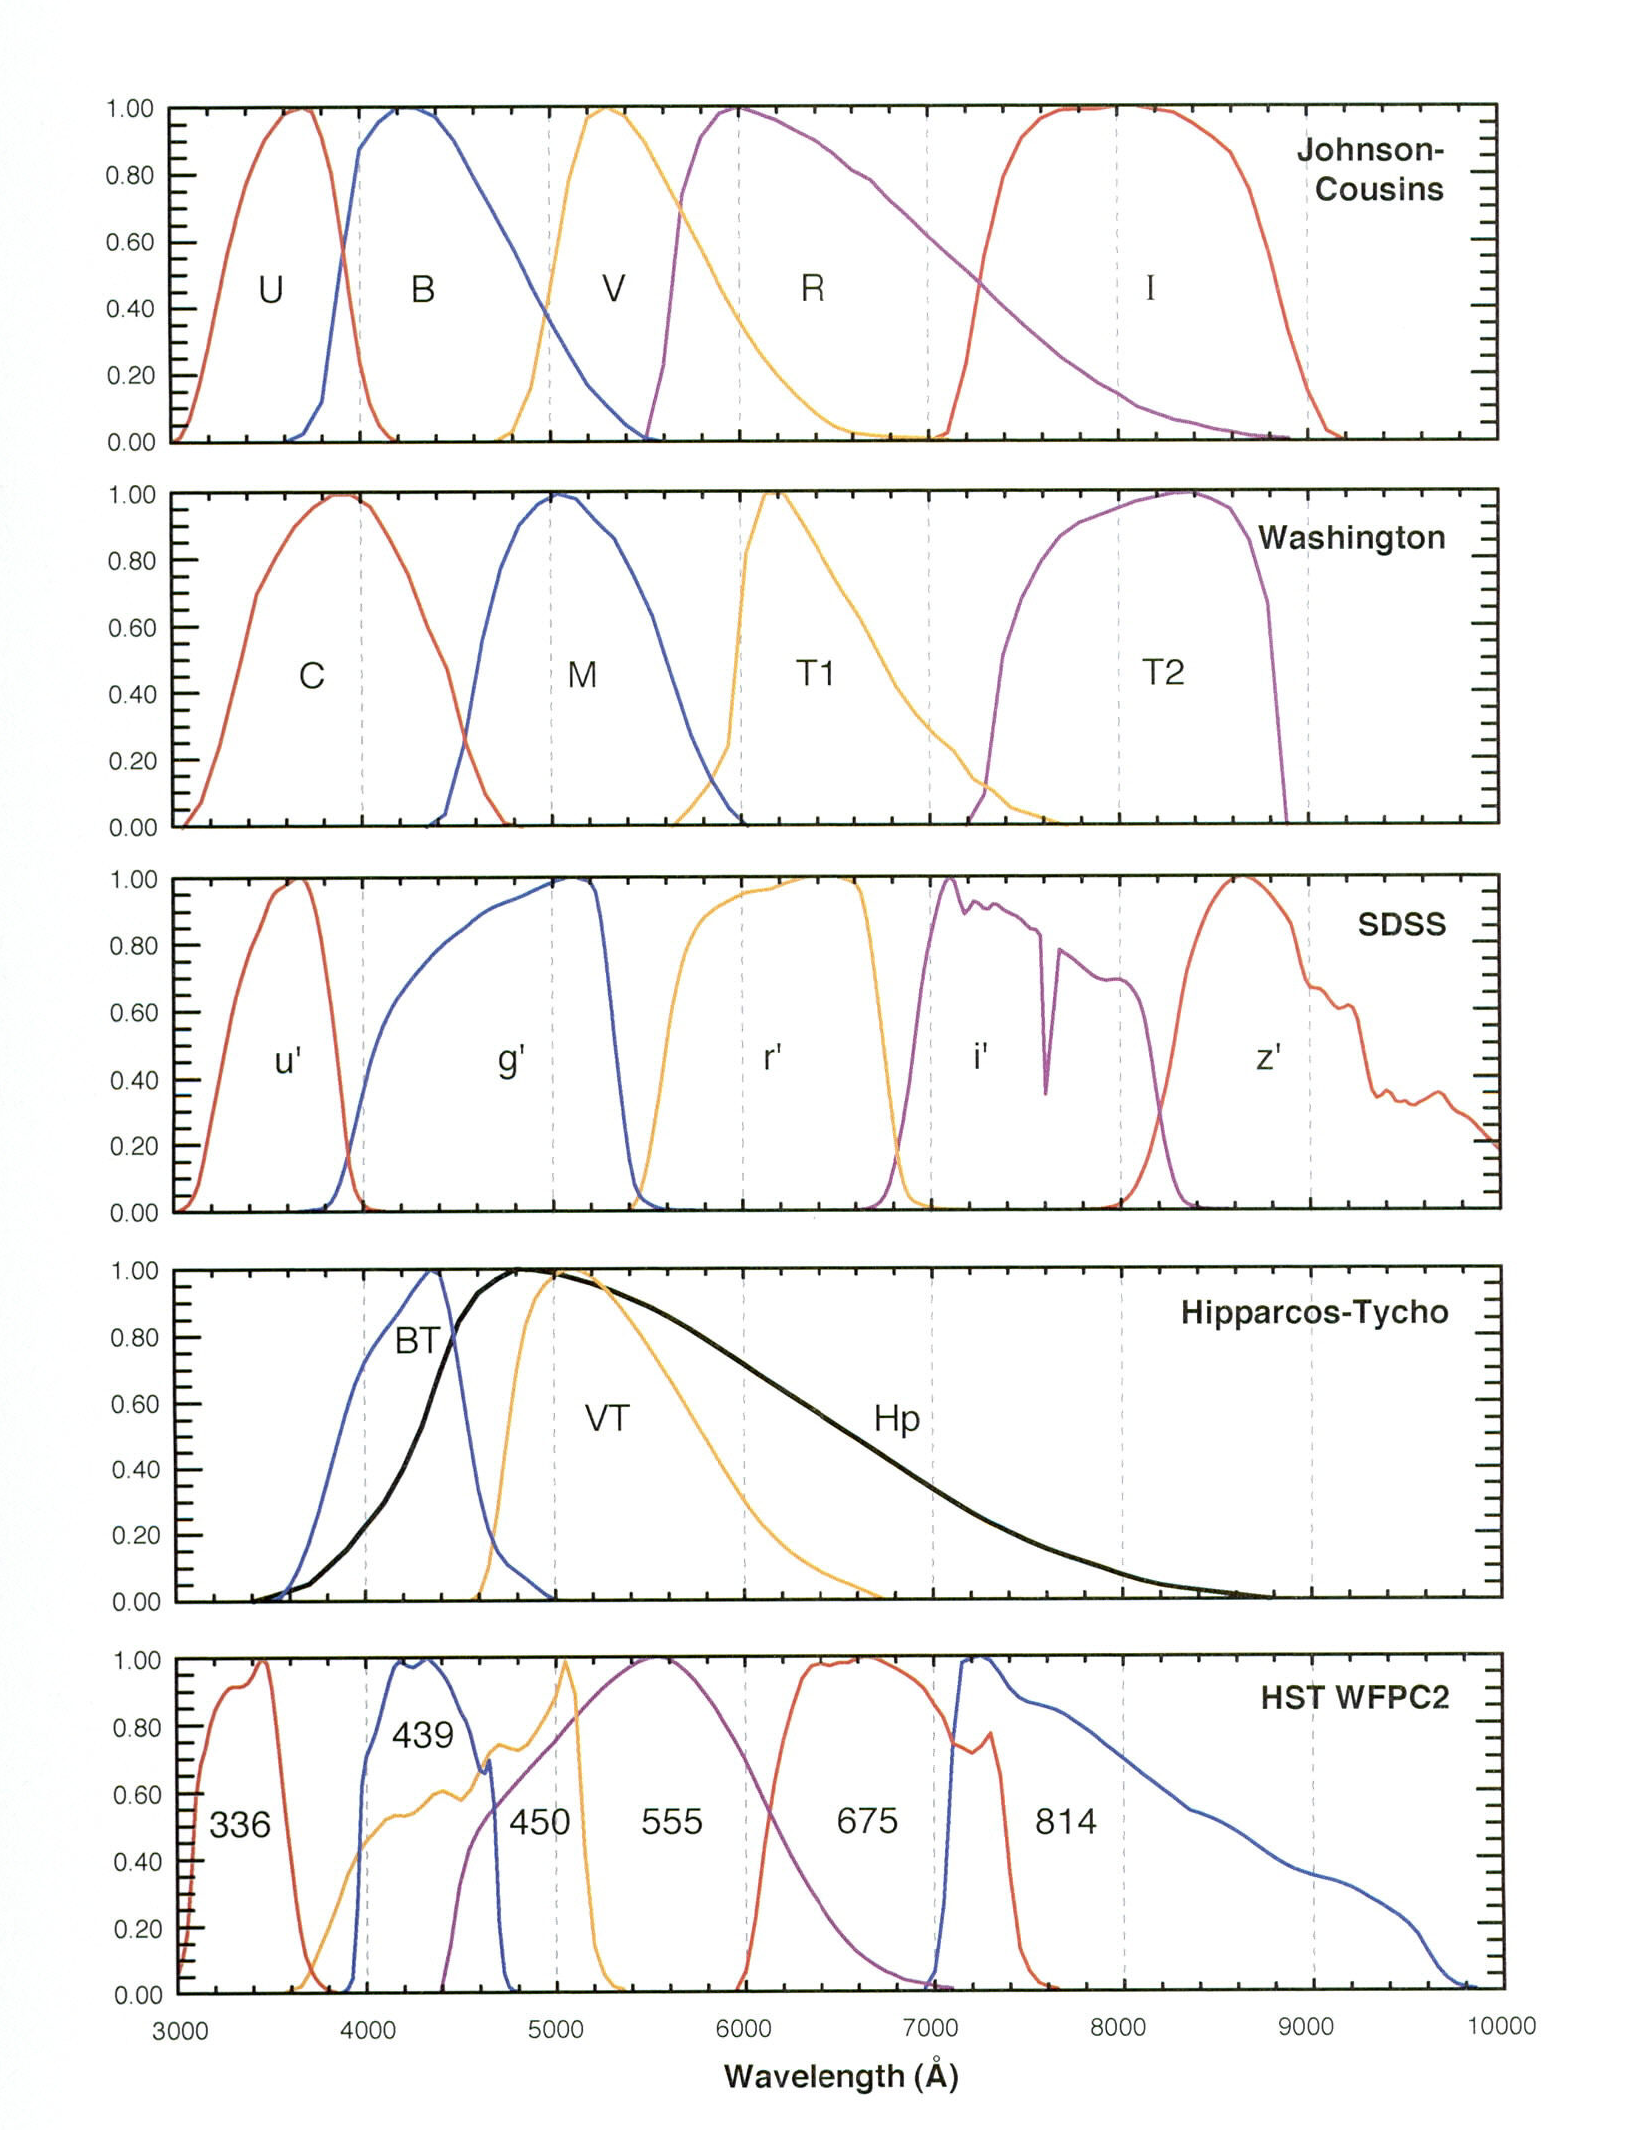
\includegraphics[width=0.8\textwidth]{img/bessell2005_fig1.png}
	\caption[Curvas de transmisi\'on de sistemas fotom\'etricos de banda ancha]{Curvas de transmisi\'on esquem\'aticas de varios sistemas fotom\'etricos de banda ancha, incluyendo el sistema Johnson--Cousins ($UBVRI$, panel superior) empleado por OGLE. Reproducida de \citet{Bessell2005}.}
	\label{fig:bessell-filtros}
\end{figure}

\backmatter

\footnotesize
\bibliographystyle{aa_url}
\bibliography{global}

\end{document}
